%%% The main file. It contains definitions of basic parameters and includes all other parts.

%% Settings for single-side (simplex) printing
% Margins: left 40mm, right 25mm, top and bottom 25mm
% (but beware, LaTeX adds 1in implicitly)
% \documentclass[12pt,a4paper]{report}
% \setlength\textwidth{145mm}
% \setlength\textheight{247mm}
% \setlength\oddsidemargin{15mm}
% \setlength\evensidemargin{15mm}
% \setlength\topmargin{0mm}
% \setlength\headsep{0mm}
% \setlength\headheight{0mm}
% % \openright makes the following text appear on a right-hand page
% \let\openright=\clearpage

%% Settings for two-sided (duplex) printing
\documentclass[12pt,a4paper,twoside,openright]{report}
\setlength\textwidth{145mm}
\setlength\textheight{247mm}
\setlength\oddsidemargin{14.2mm}
\setlength\evensidemargin{0mm}
\setlength\topmargin{0mm}
\setlength\headsep{0mm}
\setlength\headheight{0mm}
\let\openright=\cleardoublepage

%% Generate PDF/A-2u
\usepackage[a-2u]{pdfx}

%% Character encoding: usually latin2, cp1250 or utf8:
\usepackage[utf8]{inputenc}

%% Prefer Latin Modern fonts
\usepackage{lmodern}

%% Further useful packages (included in most LaTeX distributions)
\usepackage{amsmath}        % extensions for typesetting of math
\usepackage{amsfonts}       % math fonts
\usepackage{amsthm}         % theorems, definitions, etc.
\usepackage{bbding}         % various symbols (squares, asterisks, scissors, ...)
\usepackage{bm}             % boldface symbols (\bm)
\usepackage{graphicx}       % embedding of pictures
\usepackage{fancyvrb}       % improved verbatim environment
\usepackage{natbib}         % citation style AUTHOR (YEAR), or AUTHOR [NUMBER]
\usepackage[nottoc]{tocbibind} % makes sure that bibliography and the lists
			    % of figures/tables are included in the table
			    % of contents
\usepackage{dcolumn}        % improved alignment of table columns
\usepackage{booktabs}       % improved horizontal lines in tables
\usepackage{paralist}       % improved enumerate and itemize
\usepackage[usenames]{xcolor}  % typesetting in color
%\usepackage{epstopdf} 
\usepackage{mhchem} 
\usepackage{chemfig} 
\usepackage[obeyFinal]{easy-todo}
\usepackage[T1]{fontenc}
\usepackage[english]{babel}
\usepackage{subfig}
%\usepackage{titlesec}  % possible modifications of sections/titles typesetting


%% some hyphenation patterns
\hyphenation{char-ged phos-pha-ti-dyl-eth-an-ol-a-mi-ne phos-pha-ti-dyl-se-ri-ne}
\tolerance=2000


%%% Basic information on the thesis

% Thesis title in English (exactly as in the formal assignment)
\def\ThesisTitle{Simulation of processes in cellular membranes}

% Author of the thesis
\def\ThesisAuthor{Josef Melcr}

% Year when the thesis is submitted
\def\YearSubmitted{2018}

% Name of the department or institute, where the work was officially assigned
% (according to the Organizational Structure of MFF UK in English,
% or a full name of a department outside MFF)
\def\Department{Institute of Organic Chemistry and Biochemistry v.v.i., AS CR}

% Is it a department (katedra), or an institute (ústav)?
\def\DeptType{Institute}

% Thesis supervisor: name, surname and titles
\def\Supervisor{prof. Pavel Jungwirth}

% Supervisor's department (again according to Organizational structure of MFF)
\def\SupervisorsDepartment{Department of physical and macromolecular chemistry}

% Study programme and specialization
\def\StudyProgramme{Physics}
\def\StudyBranch{Biophysics, chemical and macromolecular physics}

% An optional dedication: you can thank whomever you wish (your supervisor,
% consultant, a person who lent the software, etc.)
\def\Dedication{%
\todo{ TODO: Dedication. }
}

% Abstract (recommended length around 80-200 words; this is not a copy of your thesis assignment!)
\def\Abstract{%
Many important processes in cells involve ions --
fusion of synaptic vesicles with neuronal cell membranes 
is controlled by a divalent cation \ce{Ca^{2+}};
the exchange of \ce{Na^+} and \ce{K^+}
drives the the fast electrical signal transmittion in neurons. 
We have investigated model phospholipid membranes and their interactions 
with these biologically relevant ions. 
Using state-of-the-art molecular dynamics simulations,
we accurately quantified their respective affinites 
towards neutral and negatively charged phospholipid bilayers. 
In order to achieve that,
we developed a new model of phospholipids termed ECC-lipids,
which accounts for the electronic polarization
via electronic continuum correction. 
Our simulations with this new force field 
reach for the first time a quantitative agreement 
with the experimental lipid electrometer concept 
for POPC and also for POPS with all the studied cations. 
We have also examined the effects of transmembrane voltage on phospholipid bilayers. 
The electric field induced by the voltage 
exists exclusively in the hydrophobic region of the membrane,
where it has an almost constant strength. 
This field affects the structure of nearby water molecules 
highligting its importance in electroporation. 
}

% 3 to 5 keywords (recommended), each enclosed in curly braces
\def\Keywords{%
 {molecular dynamics simulations}, {molecular modeling}, {polarizability},
{biological membranes}, {phospholipid bilayers}, {phosphatidylcholine}
{transmembrane potential},
{sodium}, {potassium}, {calcium}
}

%% The hyperref package for clickable links in PDF and also for storing
%% metadata to PDF (including the table of contents).
%% Most settings are pre-set by the pdfx package.
\hypersetup{unicode}
\hypersetup{breaklinks=true}

% Definitions of macros (see description inside)
%%% This file contains definitions of various useful macros and environments %%%
%%% Please add more macros here instead of cluttering other files with them. %%%

%%% Minor tweaks of style

% These macros employ a little dirty trick to convince LaTeX to typeset
% chapter headings sanely, without lots of empty space above them.
% Feel free to ignore.
\makeatletter
\def\@makechapterhead#1{
  {\parindent \z@ \raggedright \normalfont
   \Huge\bfseries \thechapter. #1
   \par\nobreak
   \vskip 20\p@
}}
\def\@makeschapterhead#1{
  {\parindent \z@ \raggedright \normalfont
   \Huge\bfseries #1
   \par\nobreak
   \vskip 20\p@
}}
\makeatother

% This macro defines a chapter, which is not numbered, but is included
% in the table of contents.
\def\chapwithtoc#1{
\chapter*{#1}
\addcontentsline{toc}{chapter}{#1}
}

% Draw black "slugs" whenever a line overflows, so that we can spot it easily.
\overfullrule=1mm

%%% Macros for definitions, theorems, claims, examples, ... (requires amsthm package)

\theoremstyle{plain}
\newtheorem{thm}{Theorem}
\newtheorem{lemma}[thm]{Lemma}
\newtheorem{claim}[thm]{Claim}

\theoremstyle{plain}
\newtheorem{defn}{Definition}

\theoremstyle{remark}
\newtheorem*{cor}{Corollary}
\newtheorem*{rem}{Remark}
\newtheorem*{example}{Example}

%%% An environment for proofs

%%% FIXME %%% \newenvironment{proof}{
%%% FIXME %%%   \par\medskip\noindent
%%% FIXME %%%   \textit{Proof}.
%%% FIXME %%% }{
%%% FIXME %%% \newline
%%% FIXME %%% \rightline{$\square$}  % or \SquareCastShadowBottomRight from bbding package
%%% FIXME %%% }

%%% An environment for typesetting of program code and input/output
%%% of programs. (Requires the fancyvrb package -- fancy verbatim.)

\DefineVerbatimEnvironment{code}{Verbatim}{fontsize=\small, frame=single}

%%% The field of all real and natural numbers
\newcommand{\R}{\mathbb{R}}
\newcommand{\N}{\mathbb{N}}

%%% Useful operators for statistics and probability
\DeclareMathOperator{\pr}{\textsf{P}}
\DeclareMathOperator{\E}{\textsf{E}\,}
\DeclareMathOperator{\var}{\textrm{var}}
\DeclareMathOperator{\sd}{\textrm{sd}}

%%% Transposition of a vector/matrix
\newcommand{\T}[1]{#1^\top}

%%% Various math goodies
\newcommand{\goto}{\rightarrow}
\newcommand{\gotop}{\stackrel{P}{\longrightarrow}}
\newcommand{\maon}[1]{o(n^{#1})}
\newcommand{\abs}[1]{\left|{#1}\right|}
\newcommand{\dint}{\int_0^\tau\!\!\int_0^\tau}
\newcommand{\isqr}[1]{\frac{1}{\sqrt{#1}}}

%%% Various table goodies
\newcommand{\pulrad}[1]{\raisebox{1.5ex}[0pt]{#1}}
\newcommand{\mc}[1]{\multicolumn{1}{c}{#1}}


%%%%%%%%%%%%%%%%%%%%%%%%%%%%%%%%%%%%%%%
%%%%%%%%%%%%%%%%%%%%%%%%%%%%%%%%%%%%%%%
% Title page and various mandatory informational pages
\begin{document}

%%% Custom variables
% width suitable for fitting into a column in 1-column page layout
\newlength{\figwidth}
\setlength{\figwidth}{9 cm} 
\newlength{\figwidthsmall}
\setlength{\figwidthsmall}{6 cm} 
\newlength{\figwidthfull}
\setlength{\figwidthfull}{14 cm} 

%%%%%%%%%%%%%%%%%%%%%%%%%%%%%%%%%%%%%%%
%%% Title page of the thesis and other mandatory pages

%%% Title page of the thesis

\pagestyle{empty}
\hypersetup{pageanchor=false}
\begin{center}

\centerline{\mbox{
\includegraphics[width=166mm]{../img/logo-en.pdf}}}

\vspace{-8mm}
\vfill

{\bf\Large DOCTORAL THESIS}

\vfill

{\LARGE\ThesisAuthor}

\vspace{15mm}

{\LARGE\bfseries\ThesisTitle}

\vfill

\Department

\vfill

\begin{tabular}{rl}

Advisor of the thesis: & \Supervisor \\
\noalign{\vspace{2mm}}
Study programme: & \StudyProgramme \\
\noalign{\vspace{2mm}}
Study branch: & \StudyBranch \\
\end{tabular}

\vfill

% Zde doplňte rok
Prague \YearSubmitted

\end{center}

\newpage

%%% Here should be a bound sheet included -- a signed copy of the "doctoral
%%% thesis assignment". This assignment is NOT a part of the electronic
%%% version of the thesis. DO NOT SCAN.

%%% A page with a solemn declaration to the doctoral thesis

\openright
\hypersetup{pageanchor=true}
\pagestyle{plain}
\pagenumbering{roman}
\vglue 0pt plus 1fill

\noindent
I declare that I carried out this doctoral thesis independently, and only with the cited
sources, literature and other professional sources.

\medskip\noindent
I understand that my work relates to the rights and obligations under the Act No.~121/2000 Sb.,
the Copyright Act, as amended, in particular the fact that the Charles
University has the right to conclude a license agreement on the use of this
work as a school work pursuant to Section 60 subsection 1 of the Copyright Act.

\vspace{10mm}

\hbox{\hbox to 0.5\hsize{%
In ........ date ............	% FIXME!
\hss}\hbox to 0.5\hsize{%
signature of the author
\hss}}

\vspace{20mm}
\newpage

%%% Dedication

\openright

\noindent
\Dedication

\newpage

%%% Mandatory information page of the thesis

\openright

\vbox to 0.5\vsize{
\setlength\parindent{0mm}
\setlength\parskip{5mm}

Title:
\ThesisTitle

Author:
\ThesisAuthor

\DeptType:
\Department

Advisor:
\Supervisor, \SupervisorsDepartment

Abstract:
\Abstract

Keywords:
\Keywords

\vss}

\newpage

\openright
\pagestyle{plain}
\pagenumbering{arabic}
\setcounter{page}{1}


%%% A page with automatically generated table of contents of the doctoral thesis

\tableofcontents

%%% Each chapter is kept in a separate file
\chapter*{Preface}
\addcontentsline{toc}{chapter}{Preface}

Cellular membranes are important and evolutionarily very old biological structures. 
\citep{MolBiolCell, Knudsen_book2002} 
The first primitive predecessors of cells already bear hints of membranes 
separating their inner environment from the outer world. 
Current organisms often contain a multitude of immensly complex membranes, 
each serving many functions. 
\emph{Processes in cellular membranes} are crucial for life. 

%In this thesis,
%Simulation of processes in cellular membranes,
%I focus on the processes, 
My work is motivated by the processes,
which involve interactions of biologically relevant ions with membranes. 
Excitable cells like neurons 
rely on the exchange of the monovalent cations \ce{Na^+} and \ce{K^+}
enabling them to conduct electrical signals. 
Fusion of synaptic vesicles with neuronal cell membranes 
is controlled by a divalent cation \ce{Ca^{2+}}.
In this work, 
I accurately quantify the interactions of these cations, 
i.e.,
\ce{Na^+}, \ce{K^+} and \ce{Ca^{2+}},
with model biological membranes
using classical molecular dynamics simulation. 
In order to achive this goal,
I developed an improved force field
of phospholipids as the major components of cellular membranes.
These models account for electronic polarization
using the electronic continuum correction,  
which is an effective way of accounting for electronic polarization via charge rescaling. 
My simulations provide a proof of concept 
for the applicability of this approach 
to both neutral and charged lipids. 
I demonstrate that accounting for electronic polarization 
is necessary for accurate description of interactions 
between ions and phospholipids. 

%==============================
Extend with the transmembrane potential modeling work.
%==============================

\chapter{Biological membranes}
\label{chap:intro}

 \textbf{Basically brief recap of preface enriched with extras on membranes.}

 Introduction to the field. 
 Inner/outer environment. 
 Membrane separates and helps maintaining non-equilibrium unequal distributions of cations/electrolytes. 

 Interaction with cations and its significance -- already in preface?

 Exemplify things with the following: \\
 Processes in Neurons. 
 Transmembrane potential. 
 Action potential. 

\section{Membrane components}

\subsection{Phospholipids}

\subsection{Cholesterol}

\subsection{Other lipids: Myelination -- chop into a short enrichment -- a particular composition}
Myelin has two important advantages:\textbf{ fast conduction speed and energy efficiency}. For axons larger than a minimum diameter (roughly 1 micrometre), myelination increases the conduction velocity of an action potential, typically tenfold. Conversely, for a given conduction velocity, myelinated fibers are smaller than their unmyelinated counterparts. For example, action potentials move at roughly the same speed (25 m/s) in a myelinated frog axon and an unmyelinated squid giant axon, but the frog axon has a roughly 30-fold smaller diameter and 1000-fold smaller cross-sectional area. Also, since the ionic currents are confined to the nodes of Ranvier, far fewer ions "leak" across the membrane, saving metabolic energy. This saving is a significant selective advantage, since the human nervous system uses approximately 20\% of the body's metabolic energy.

In nature, myelinated segments are generally long enough for the passively propagated signal to travel for at least two nodes while retaining enough amplitude to fire an action potential at the second or third node. Thus, the safety factor of saltatory conduction is high, allowing transmission to bypass nodes in case of injury. However, action potentials may end prematurely in certain places where the safety factor is low, even in unmyelinated neurons; a common example is the branch point of an axon, where it divides into two axons.

\subsection{Non-lipids: protein and sugar, glycocalyx}

\section{Model membranes, Phospholipid bilayers }

 Model membranes and membrane models in experiments and in simulations.
 Phospholipid bilayers or just bilayers with various composition. 

 Supported bilayers, vesicles, SUV, LUV, GUV, multilamellar vesicles




\section{Interactions of cations with phospholipid bilayers}

 Several chosen Experimental studies. 

 Contradiction between simulation/experimental studies 
 (use what's in the paper PCCP NMRLipids II). 

Due to its high physiological importance --- nerve cell signalling being the prime example ---
interaction of cations with phospholipid membranes
has been widely studied via theory, simulations, and experiments.
The relative ion binding affinities are generally agreed to
follow the Hofmeister series~\cite{eisenberg79,cevc90,tocanne90,binder02,celma07,leontidis09,vacha09a,klasczyk10,harb13}, 
however,
consensus on the quantitative affinities is currently lacking.
Until 1990, the consensus (documented in two extensive reviews~\cite{cevc90,tocanne90}) was that
while  multivalent cations interact significantly with phospholipid bilayers,
for monovalent cations (with the exception of Li$^+$) the interactions are weak.
This conclusion has since been strengthened by further
studies showing that bilayer properties remain unaltered upon the addition of sub-molar concentrations of monovalent 
salt~\cite{binder02,pabst07,filippov09}.
Since 2000, however, another view has emerged, suggesting much stronger interactions between phospholipids and monovalent cations, and strong Na$^{+}$ binding in particular~\cite{bockmann03,bockmann04,vacha09a,manyes05,manyes06,fukuma07,leontidis09,ferber11,morata12,klasczyk10,harb13}.

The pre-2000 view has the experimental support that
(in contrast to the significant effects caused by any multivalent cations)
sub-molar concentrations of NaCl have a negligible effect on
phospholipid infrared spectra~\cite{binder02},
area per molecule~\cite{pabst07},
dipole potential~\cite{clarke99},
lateral diffusion~\cite{filippov09},
and choline head group order parameters~\cite{akutsu81};
in addition, the water sorption isotherm of a NaCl--phospholipid system
is highly similar to that of a  pure NaCl solution
--- indicating that the ion--lipid interaction is very weak~\cite{binder02}. 

The post-2000 'strong binding' view rests on experimental and above all simulational findings.
At sub-molar NaCl concentrations, the rotational and translational dynamics of membrane-embedded fluorescent probes decreased~\cite{bockmann03,vacha09a,harb13}, and atomic force microscopy (AFM) experiments showed changes in bilayer hardness~\cite{manyes05,manyes06,fukuma07,ferber11,morata12};
in atomistic molecular dynamics (MD) simulations, phospholipid bilayers consistently bound Na${^+}$,
although the binding strength depended on the model used~\cite{bockmann03,bockmann04,sachs04,berkowitz06,cordomi08,cordomi09,valley11,berkowitz12}.

Some observables have been interpreted in favour of both views. For example,
as the effect of monovalent ions (except Li$^+$)  on the phase transition temperature is tiny
(compared to the effect of multivalent ions), it was initially interpreted 
as an indication that only multivalent ions and Li$^+$ specifically bind to phospholipid bilayers~\cite{cevc90}; 
however, such a small effect in calorimetric measurements was later interpreted to indicate that also
Na$^+$ binds~\cite{bockmann03,klasczyk10}.
Similarly, the lack of significant positive electrophoretic mobility
of phosphatidylcholine (PC) vesicles in the presence of NaCl
(again in contrast to multivalent ions and Li$^+$)
suggested weak binding of Na$^+$~\cite{eisenberg79,tatulian87,manyes05,manyes06,klasczyk10};
%NaCl increases the (initially negative) zeta potential to only about zero,
%whereas positive zeta potentials are generally reached with
however, these data were also explained by a countering effect of the Cl$^-$ ions~\cite{berkowitz06,knecht13}.
Furthermore, to reduce the area per lipid in scattering experiments, molar concentrations of NaCl were required~\cite{pabst07}, indicating weak ion--lipid interaction;
in MD simulations, however, already orders of magnitude lower concentrations resulted in Na$^+$ binding and a clear reduction of area per lipid~\cite{bockmann03,cordomi08}.
Finally, lipid lateral diffusion was unaltered by NaCl in noninvasive NMR experiments~\cite{filippov09};
%suggesting that the fluorescence results arise from Na$^{+}$ interactions with probes rather than with lipids.
%This is pointed out in Conclusions, which I think is the best place for it. -markus.
however, as it was reduced upon Na$^+$ binding in simulations,
the reduced lateral diffusion of fluorescent probes~\cite{bockmann03,vacha09a,harb13}
has been interpreted to support the post-2000 'strong binding' view.

In this paper, we set out to solve the apparent contradictions
between the pre-2000 and post-2000 views.
To this end, we employ the 'molecular electrometer' concept,
according to which the changes in the C--H order parameters of the $\alpha$ and $\beta$ carbons 
in the phospholipid head group (see Fig.~\ref{POPCstructure}) can be used to measure the ion affinity for a
PC lipid bilayer~\cite{brown77,akutsu81,altenbach84,seelig87,scherer89}.
As the order parameters can be accurately measured in experiments and directly compared to 
simulations~\cite{ollila16}, applying the molecular electrometer as a function of cation concentration allows the 
comparison of binding affinity between simulations and experiments.
In addition to demonstrating the usefulness of this general concept,
we show that the response of the $\alpha$ and $\beta$ order parameters to penetrating cations
is qualitatively correct in MD simulations, but that in several  models the affinity of Na$^{+}$ for PC bilayers
is grossly overestimated.
Moreover, we show that the accuracy of lipid--Ca$^{2+}$ interactions 
in current models is not enough for atomistic resolution interpretation of NMR experiments. 


\section{NMR order parameter measurements}
 
  More general statements about NMR  -- especially the way $S_{CH}$ is measured. 

\subsection{Electrometer concept} \label{section:electrometer} 

Comparing MD simulation to NMR experiments, we can validate the ion 
binding affinity in lipid bilayer simulations using the 'electrometer concept'~ \citep{seelig87, catte16}. 
This method is based on the experimental observation that the C-H bond order parameters of $\alpha$ and $\beta$ carbons in a PC lipid head group (Fig.~\ref{simVSexpNOions}) are proportional to the amount of charge bound per lipid~\citep{seelig87}. 
The order parameters for all C-H bonds in lipid molecules can be accurately measured using $^2$H NMR or $^{13}$C NMR techniques \citep{ollila16}. 
From MD simulations the order parameters can be calculated using the relation 
\begin{equation}\label{OP} 
S_{\rm CH}=\frac{1}{2}\langle 3\cos^2\theta -1 \rangle, 
\end{equation} 
where $\theta$ is the angle between the C-H bond and the membrane normal. 
Angular brackets point to the average over all sampled configurations. 
 
The relation between the amount of the bound charge per lipid, $X^\pm$, and the head group order parameter change, $\Delta S_{\rm{CH}}^{i}$, is empirically quantified as~\citep{seelig87,ferreira16} 
\begin{equation}\label{OPchangeEQ} 
\Delta S_{\rm{CH}}^{i}= S_{\rm{CH}}^{i}(X^\pm)-S_{\rm{CH}}^{i}(0) \approx m_i \frac{4 }{3\chi}X^\pm, 
\end{equation} 
where $i$ refers to either the $\alpha$ or $\beta$ carbons, $S_{\rm{CH}}^{i}(0)$ denotes the order parameter in the absence of bound charge, $\chi$ is the quadrupole coupling constant ($\chi \approx$\,167\,kHz), and $m_i$ is an empirical constant depending on the valency and location of the bound charge. 
 
 
The measured change of the order parameter depends on the head group response to the bound charge and on the amount of the bound charge (\textit{i.e.,} $m_i$ and $X^\pm$ in Eq.~\ref{OPchangeEQ}, respectively).  
The empirical factor $m_i$ has to be adequately quantified before the electrometer concept can be used to analyze the binding affinities. 
This calibration has been done experimentally for a wide range of systems~\citep{seelig87, beschiasvili91}. 
To calibrate the response of the head group order parameters to the bound charge in simulations, we use experimental data for a strong cationic surfactant dihexadecyldimethylammonium bromide  (DHAB) mixed with a POPC bilayer~\citep{scherer89}. DHAB\\[0.5cm] 
%\vspace{0.5cm} 
%\chemfig{ -[:0,3.5,,,draw=none]\chemabove{N}{\scriptstyle\oplus} (-[:150]H_3C)(-[:210]H_3C)(-[:330]{(}CH_2{)}_{15}-CH_3)(-[:30]{(}CH_2{)}_{15}-CH_3) }   
%\vspace{0.5cm} \\ 
is a cationic surfactant having two acyl chains and bearing a unit charge at the hydrophilic end. 
Due to its structure it is expected to locate in the bilayer similarly to the phospholipids and its molar ratio then gives directly the amount of bound unit charge per lipid $X^\pm$ in these systems~\citep{scherer89}. 
 





\chapter{Molecular modeling of biological membranes}
\label{chap:methods}

Biological membranes are of a great interest in biology and biophysics. 
The tools and methods that enable their research have greatly evolved over the last decades. 
Nowadays, there is a plethora of membrane models and experimental methods, 
each having its benefits and drawbacks \citep{REF} \todoi{1-2 chosen reviews, everything else in prev chapter}
(see section~\ref{sec:modelmemb} in chapter~\ref{chap:intro} for a detailed overview). 

Molecular simulation can be considered as one of the newer approaches in this field. 
Starting with simple membrane models \citep{REF} \todoi{REF: few old/new simulation works},
simulation of membranes has evolved into a field of computational biophysics
that is capable of answering fundamental questions.
The recent progress in computational resources and algorithms
has allowed the simulations to grow in spatial scales and composition complexity
bringing more relevance for applications in biology. \citep{REF: CECAM workshop} \todoi{REF to CECAM workshop 2018 Lugano}

Molecular dynamics simulations of biological membranes employ classical particle-based models of molecules. 
Vast majority of the models are built using classical non-polarizable particles, 
each representing an individual atom (atomistic models), 
or a group of atoms (united-atom or coarse grained models). 
The following classical models belong among the most succesful:
\begin{itemize}
 \item Atomistic
 \begin{itemize}
   \item CHARMM \citep{klauda10}
   \item Slipids \citep{jambeck12, jambeck12b}
   \item OPLS lipids by \citet{maciejewski14}
   \item Lipid14 \citep{dickson14}
  \end{itemize}

 \item Coarse grained
 \begin{itemize}
   \item MARTINI \citep{marrink07}
   \item Berger \citep{Berger97}
   \item CHARMM-UA \citep{lee14}
  \end{itemize}
\end{itemize}

Despite all successes and valuable insights simulations have provided, 
there is still a large room for possible improvements of the current simulation models. 
For example, recent studies by \citet{botan15, catte16} has shown 
that both structure and interaction of phospholipid models require further optimization 
in order to become capable of interpreting solid state NMR experiments. 
In particular, we have discovered that 
the lack of polarizability is a major issue in any of the models 
from the above mentioned works \citep{botan15, catte16}
when interactions with charged moieties become important. 
Several possible ways for embedding polarizability into simulations, both explicit and implicit, 
will be introduced in the following sections. 





\section{Classical molecular dynamics simulations}

Classical molecular dynamics simulation is used to provide insight into the dynamics and structure of the particles. 
\todo{Following taken from my diploma thesis directly -- to be modified!}
% Intro, Usage, boundaries (volume, time)
  Molecular dynamics simulations (MD) represent a branch of computational methodologies that can be desribed as theoretical experiments. 
  Their usage lays usually in desctiption of equilibrium states or in an assassement of evolution of non-equilibrium states.
  By running a computer simulation with subsequent application of statistical analysis, distributions of physical properties are usually obtained. 
  These methods were tradationally used in conjunction with experiments to help their interpretation and to test the theories behind both studies. After many years of development, molecular simulations are even used for prediction nowadays.

% I challenge you to a duel through time and space. 
  There are apparent advantages over experiments. Simulations can be used in cases when the experiment would be hard to accomplish; the resolution in time and space is easily reached. An evident disadvantage is, however, that the performed simulation is always only a theoretical model of a reality. 

 % Few words about propagators and how they should behave

In classical MD simulations, though, Newton equations of motion are used instead since the studied system are represented classicaly -- atoms are embodied by point masses with point partial charges; the exerting forces are defined by an approximate interaction potential (see section \ref{inter-pot}). 


   Interaction of atoms was generally described in the previous sections using an interaction potential $V$. Force fields represent one of its types.

     Force field is an empirical potential. It can be obtained by fitting a particular mathematical formula to an experiment or ab-initio calculations. It is the fastest method yet the most inaccurate. Chemistry can be made only in very special forms of it (for example EVB, empirical valence bond). It allows us to study large systems conatining tens or even hunderds of thousands atoms. More information will be given in the following sections.


  Classical force fields are pairwise additive. Amber, Charmm, OPLS, UFF and many others belong to this group. 

  Amber may serve as an example of a simple classical force field potential form:
 % Amber potential energy form:
\begin{eqnarray}  \label{amber}
  V = & \displaystyle \sum _{bonds} K_b (r-r_{eq})^2 + \sum _{angles} K_\Theta (\Theta-\Theta_{eq})^2 + \\ \nonumber
      & \displaystyle \sum _{dihedrals} \frac{1}{2} V_n (1+\cos(n\phi -\delta)) + \sum _{i<j} \left [ s_{ij} ^{VdW} \left( \frac{A_{ij}}{r_{ij} ^{12}} - \frac{B_{ij}}{r_{ij} ^6} \right ) + s_{ij}^q \frac{q_i q_j}{\epsilon \, r_{ij}} \right ]
\end{eqnarray}
  Non-bonded interaction are usually evaluated only for atoms separated by more than 3 bonds, as the interactions are already included in the bond stretching and angle bendig terms. 
  The number of non-bonded terms scales approximately quadratically with the size of the system and so it takes the most of the time of evaluation of the interaction potential.

   The core of a force field is the  definition of the potential. The mathematical form varies among different types of force fields; the harmonic potential is the most common, though, as it usually describes the potential in equilibrius position well. By fitting the formula to an experimental or ab-inition data, parameters are obtained for the various terms. Force fields for smaller systems (for example salts dissolved in water) can more precise than for larger systems, where the formula must be more general due to the high number of types of interactions. 

 When describing a molecule it's most often an advantage to use the internal coordinates. Instead of using the coupled $3N$ cartesian coordinates, the internal coordinates allow us to use the local symmetry of a molecule, which simplifies the formula. 
 These terms appear in force fields for biophysical applications most frequently: 
 bond stretching, angle bending, dihedral torsions.


  Except the bonding terms that describe the interactions of molecules separated by less than four bonds there also must be such terms that incorporate the strong electrostatic interaction and dispersion. 

  Electrostatic interaction has a long range impact meaning that its contributions from an infinite distance don't vanish and can't be neglected. A multipole expansion is used for its description: the 1\textsuperscript{st} term is a monopole (charged molecules, ions); 2\textsuperscript{ns} is a dipole that is usually present in all structures (for ex. water); 3\textsuperscript{rd} is a quadrupole etc.

  Charges on atoms are represented in that manner. The most important part plays the monopole. For that reason atoms are simplified as partial point charges. If a better precision is needed, dipoles can be added, though it's not a common case to do so. The dipole moment can be added by either specifying a dipole or by adding point charges representing it. The latter method can lead to different results due to the ambiguous determination of the representing charges. 

  As the electrostatic interaction is among the strongest even in neutral systems, its precise treatment is eminent. Ways how to deal with its long ranged nature follow in subsequent sections. 



  Ewald summation: When periodic boundary conditions for bulk compensation are used, the long range contribution to the electrostatic interaction cannot be neglected. If the system is neutral, it can be treated in a more efficient manner if the summation over distant charges is done in Fourier space rather than in real space. In a case of a charged system, the summation would not converge. 

  The procedure is that the contributions are divided into two groups depending on their distance from the center. The nearer charges are summed in real space. The further charges are formally treated as delta functions, and a gaussian curve with approximately the same but opposite charge is added to each of them. With such tuning the sum in real space becomes convergent. To compensate the added gaussians, their inversion is summed in the reciprocal Fourier space, where it converges better than in real space. 
% aplikace v programech -- fast FT, P$^3$M (par-par-particle mesh), PME, SPME (smooth PME)



  Van der Waals: When two atoms draw nearer their electronic structure changes due to electrostatic interaction and electronic correlation. As a consequence, even neutral atoms may attract each other by induced dipoles. The tendency to form them is specified by polarizability, which is a quantity that decribes the tendency of atoms to polarize themselves in an outer electric field. 

  Besides polarizibility, that was briefly introduced in previous sections, there is also a dispersion interaction that describes electronic correlation. Introduction of such forces is crucial with the point charge approximation as oppositely charged atoms would collapse into each other otherwise.

  The force is not strong; it's attractive in a distance $r$ from the source and is approximately proportional to $\frac{1}{r^6}$. The dispersion force is repulsive when atoms are near and the electronic orbital overlap a lot. This is approximately proportional to $ e^{-\alpha r} $.


  Lennard-Jones form doesn't suffer from this artefact. Accordingly to its form it is commonly reffered to as (12,6) potential:
\begin{equation}
   U_{VdW-LJ} =  \frac{A_{ij}}{r_{ij}^{12}} - \frac{B_{ij}}{r_{ij}^6} = \epsilon _{ij} \left [ \left (\frac{\sigma _{ij}}{r_{ij}} \right )^{12} - 2 \left ( \frac{\sigma _{ij}}{r_{ij}} \right )^6 \right ]
\end{equation}
  where $\epsilon$ denotes the depth of the minimum and $\sigma$ is the equilibrius position. 

  It's unusual to define parameters for every pair of atomic types in a force field. The specified parameters often refer to the interaction of two atoms of the same type. The rest of the parateres are obtained via mixing rules, which definition differs among forcefields. The most common mixing rules are Lorentz-Berthelot's:
\begin{equation}
 \sigma _{ij} = \frac{1}{2} (\sigma _{ii} + \sigma _{jj}) \, ; \quad \epsilon _{ij} = \sqrt{\epsilon _{ii} \, \epsilon _{jj}} 
\end{equation}
%\poznmini{souvisí s optikou -- index lomu }









\section{Including polarizability}

  Lit. research (history) on how people include polarizability in classical simulations. 

\subsection{Explicit treatment of electronic polarizability}

 Joint subsection on Drude particles and polarizable dipoles, the most common ways of introducing polarizability explicitly into the MD simulation. 

\subsection{Electronic continuum correction as implicit treatment of electronic polarizability}

The lack of electronic polarizability in standard MD force fields has been considered a serious issue since the early days of lipid bilayer simulations. In this work, we circumvent the demanding explicit inclusion of electronic polarization effects~\citep{lucas12, chowdhary13} by accounting for the electronic part of polarizability in lipid bilayer simulations implicitly via the electronic continuum correction (ECC)~\citep{leontyev11}. Technically, this is similar to the phenomenological charge-scaling applied in earlier studies of surfactants, lipids or ionic liquids \citep{jonsson86, egberts94, beichel14}. However, the present concept of ECC is physically well justified and has theoretical support~\citep{leontyev09, leontyev10, leontyev11, leontyev14}. 
 
According to ECC, the electronic polarizability can be included into non-polarizable MD in a mean-field way by  
embedding the ions in a homogeneous dielectric continuum with a dielectric constant $\epsilon_{el}$, which is the electronic part of the dielectric constant of the medium~\citep{leontyev11}. Following Coulomb's law,  ECC can be directly incorporated by scaling the charges with a constant scaling factor of $f_q = \epsilon _{el} ^{-1/2}$, yielding 
\begin{equation} 
Q^{ECC} = f_q \cdot Q 
\end{equation} 
for the ECC corrected charges.  
Given that the  high frequency dielectric constant of water is $\epsilon _{el} = 1.78$ (\textit{i.e.,} the square of the refraction index), the scaling factor for ions in water is roughly $f_q \approx 0.75$. This scaling factor significantly improves the accuracy of simulations of solvated ions, when quantitatively compared with neutron scattering data \citep{kohagen14,kohagen16, Pluharova2014, martinek17}. 
It is important to note that the value of the 
high frequency dielectric constant  
is around 2 for almost any biologically relevant environment \citep{leontyev11}. 
The dielectric discontinuity in a lipid bilayer thus arises only 
from the orientational polarization of the molecules, which is accounted for explicitly in standard MD simulations.  
Therefore, the same correction for the electronic polarizability can be  
applied throughout the lipid bilayer/aqueous solution interface. 
 
While using the scaling factor of $f_q = 0.75$ for ions in water is well justified in the ECC theory \citep{leontyev11}, it is not clear whether the same factor should be applied to partial charges used to describe molecules in MD models, e.g., lipids in our case \citep{leontyev14}. Unlike the total charge of an ion, atomic partial charges within molecules are not physical observables. Several computational schemes exist for the assignment of partial charges for biomolecules~\citep{Hu2007}, with the restrained electrostatic potential method (RESP) being commonly used~\citep{RESP_paper, Singh1984}. Considering that water is often included in RESP calculations or charges are refined to improve certain experimental observables, the electronic polarizability effects of the solvent may to some extent be included in standard force fields~\citep{RESP_paper, Singh1984, jorgensen96, ipolq2013, benavides17}. Thus, our application of the scaling factor, $f_q$, to existing partial charges in molecules does not necessarily follow $f_q = \epsilon _{el} ^{-1/2}$. Instead, a consistent scaling factor should lie between the value of 0.75  (\textit{i.e.,} no electronic polarizability included in the original partial charges) and 1 (\textit{i.e.,} electronic polarizability fully included in the original partial charges).  
 



\section{Implicitly polarizable classical MD models of lipids using ECC}

\textbf{ Change the following text and include PE and PS into this seciton. 
         Define ECC-lipids. Introduce all lipids in this section. }

Here we develop a ECC-POPC lipid model that accurately describes binding  
of sodium and calcium ions to the POPC  lipid bilayer.  
The Lipid14~\citep{dickson14} force field  
(available in a Gromacs format from Ref. \citep{lipid14files}) was used as a starting  
point since  
it provides the most accurate response of the head groups to ions among the available  
lipid models (see Figs.~2~and~5 in Ref.~\citep{catte16}). Additionally, the Lipid14 model  
provides relatively realistic head group, glycerol backbone, and acyl chain structures~\citep{dickson14,botan15}. 
We applied the ECC correction  
to the Lipid14 model of POPC by scaling  
partial charges of the head group, glycerol  
backbone, and carbonyl regions.  
These are the polar parts of phospholipids which can  
contribute to the cation binding.  
 
To reproduce the experimental ion binding affinities, 
we scanned possible values of the scaling factor from the interval $f_q~\in~(0.75, 1.0)$. 
The ion binding affinity was benchmarked against experiments 
using the head group order parameters and the electrometer concept \citep{seelig87,catte16}, 
as discussed more detail in the next section. 
Scaling down the partial charges reduced the ion binding affinity. 
We found the most accurate ion binding affinities with a scaling factor of $f_q = 0.8$, 
which is only slightly higher than the ECC one ($f_q=0.75$). 
Note that common empirical scaling factors for monovalent ions in water are 0.8 or
even closer to unity \citep{benavides17,skinner14,nacleps}.  In contrast, modern force fields
for ionic liquids suggest values of 0.6--0.65, which are lower than $\epsilon^{-1/2}_{el}$\citep{holm14}.
Directly applying 
the 0.8 scaling to the partial charges of the head group, the glycerol backbone, and 
the carbonyls reduced the area per lipid to 60~Å$^2$. This area is smaller than in the 
original Lipid14 model ($65.6 \pm 0.5$~Å$^2$)~\citep{dickson14} and in experiments 
(64.3~Å$^2$) \citep{kucerka11}. The decrease of the area per lipid arises from a 
reduced hydration of the lipid head group region after scaling of the partial charges, which effectively 
reduces the head group polarity. We solve this problem by slightly reducing the effective radii of 
the modified head group atoms via lowering the $\sigma$ parameters in the Lennard-Jones potential by a 
factor of $f_\sigma = 0.89$. The same approach was successfully adopted for the ECC ions in aqueous 
solutions previously \citep{kohagen14, kohagen16, Pluharova2014, martinek17}. After reducing the head group atoms $\sigma$ parameters, the area per molecule is restored to the experimental value (Table~\ref{tab:apls}).  


\subsection{Structural parameters of model membranes with ECC-lipids: Agreement with experiments} 
 
%%%%%%%%%%%%%%%%%%%%%%%%%%%%%%%%%%%%%%%%%%%%%%%%%%%%%%%%%%%%%%
% problem solved: NO line breaks in the caption!
\begin{figure}[tb!] 
  \centering 
  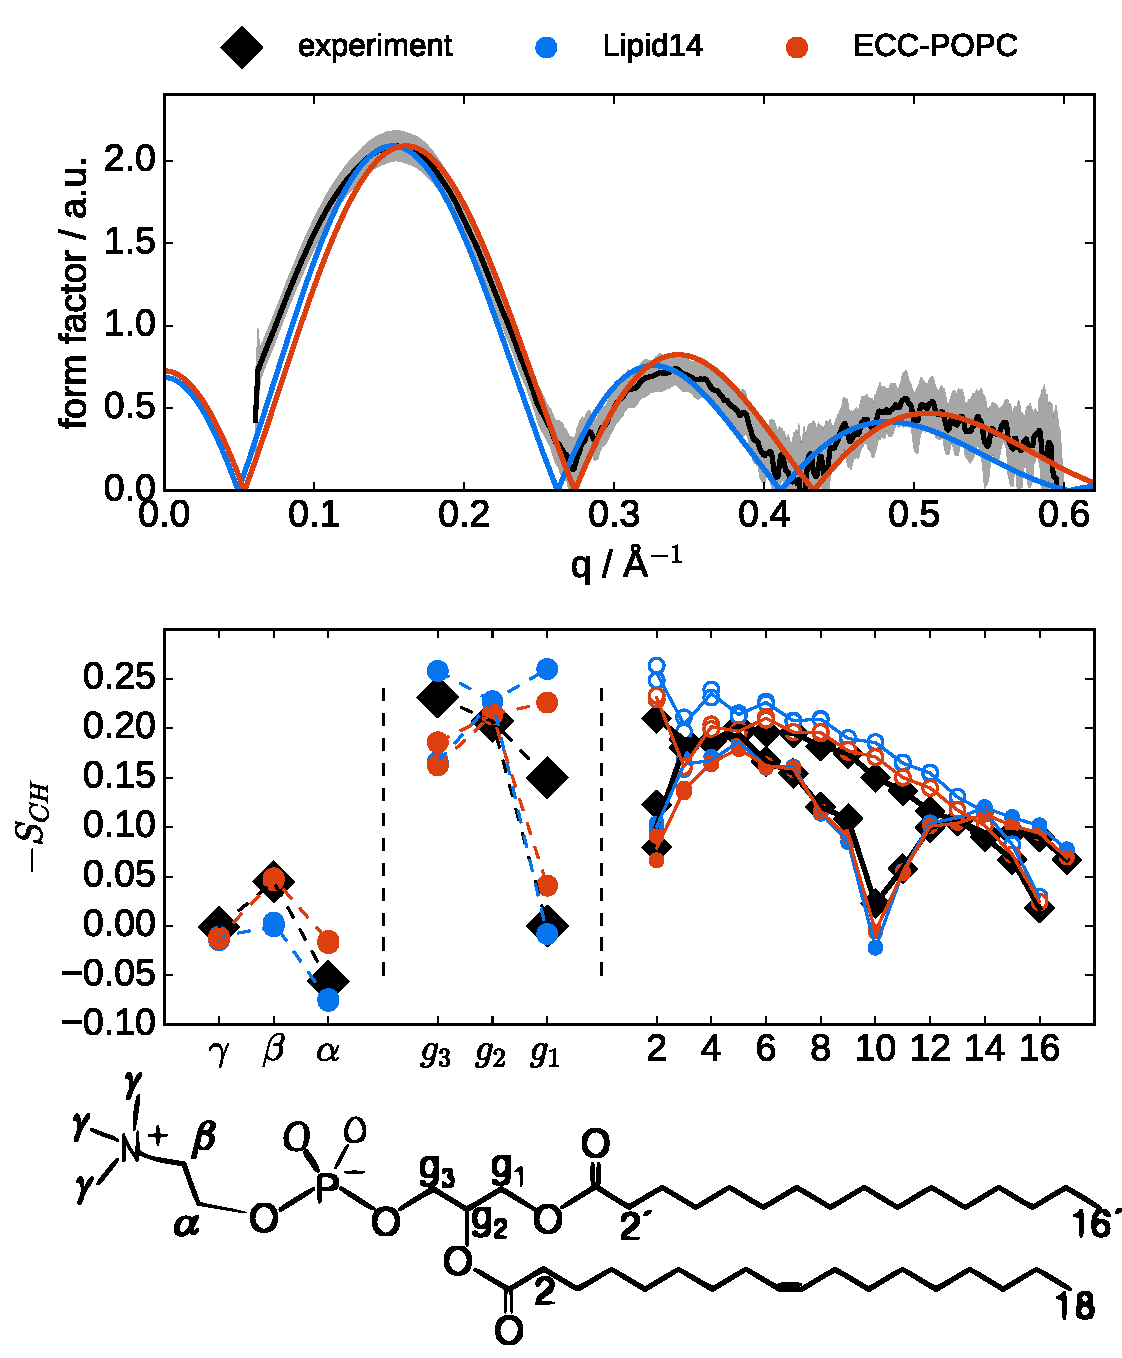
\includegraphics[width=8.2cm]{../img/ecc_popc/Order-parameters_form-factors_exp-L14-ECCL17_q80_sig89_POPC-struct.pdf} 
  \caption{ \label{simVSexpNOions} 
    Top: X-ray scattering form factors from simulations with the Lipid14 \citep{dickson14} and 
    the ECC-POPC models compared with experiments~\citep{kucerka11} at 303~K. 
    Middle: Order parameters of POPC head group, glycerol backbone and acyl chains  
    from simulations with the Lipid14 \citep{dickson14} and the ECC-POPC models 
    compared with experiments \citep{ferreira13} at 300~K. 
    The size of the markers for the head group order parameters correspond to 
    the error estimate $\pm 0.02$ for experiments \citep{botan15,ollila16}, 
    while the error estimate for simulations is $\pm 0.005$
    (Bayesian estimate of 95\% confidence interval \citep{scipy}).
    The size of the points for acyl chains are decreased by a factor of 3 to improve the clarity of the plot.
    Open/closed symbols are used for palmitoyl/oleoyl chains of POPC. 
    Bottom: The chemical structure of POPC and the labeling of the carbon segments. 
  }  
\end{figure} 


\begin{figure}[tb!] 
  \centering 
  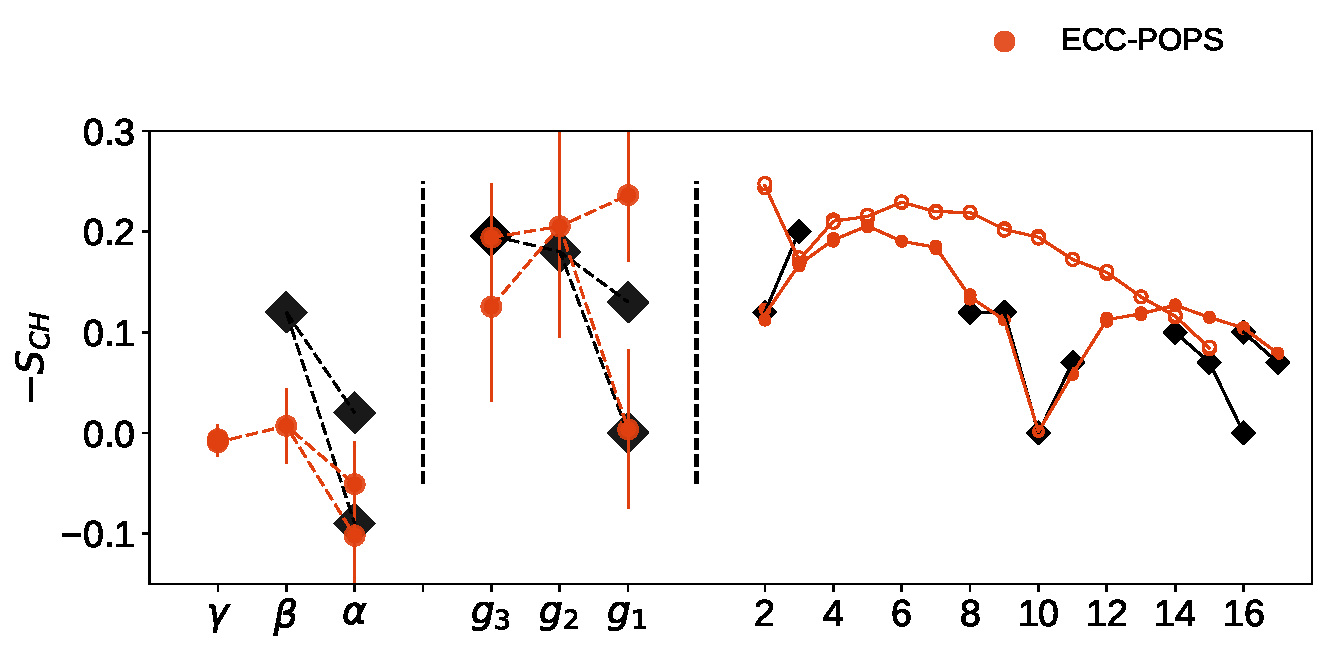
\includegraphics[width=\figwidth]{../img/ecc_pops/order_parameters_actual_pure-POPS.pdf} 
  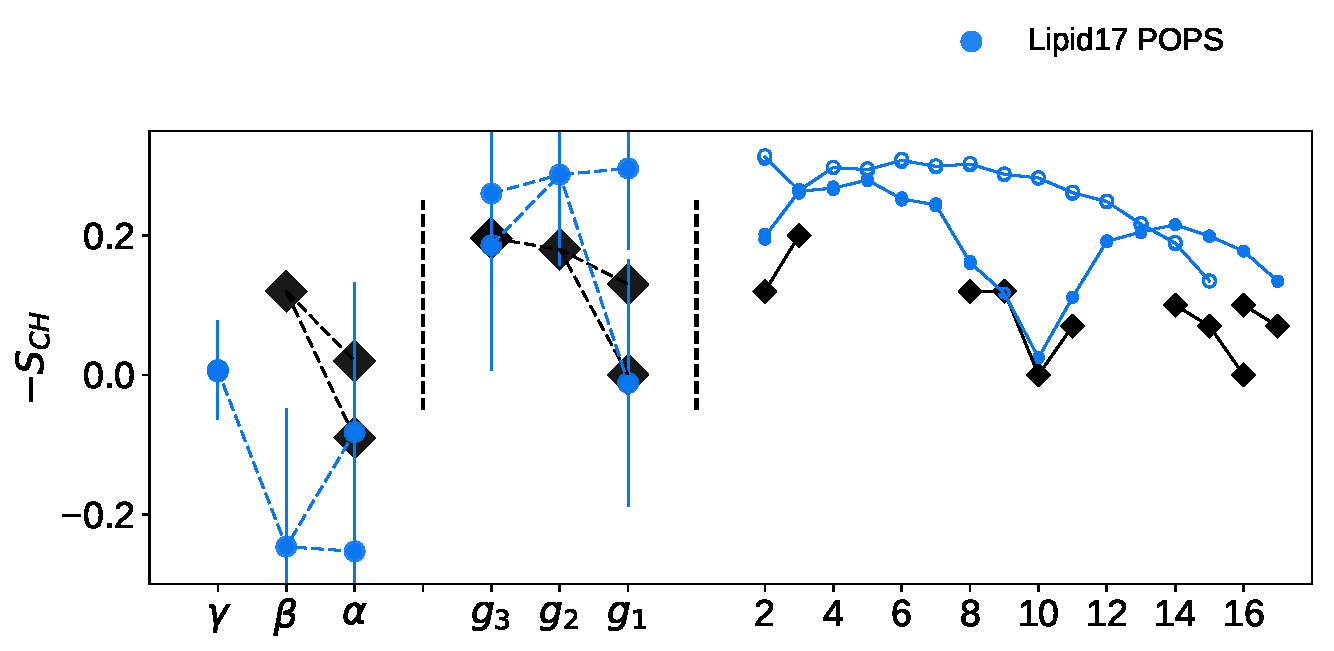
\includegraphics[width=\figwidth]{../img/ecc_pops/l17/order_parameters_actual_pure-POPS.pdf} 
  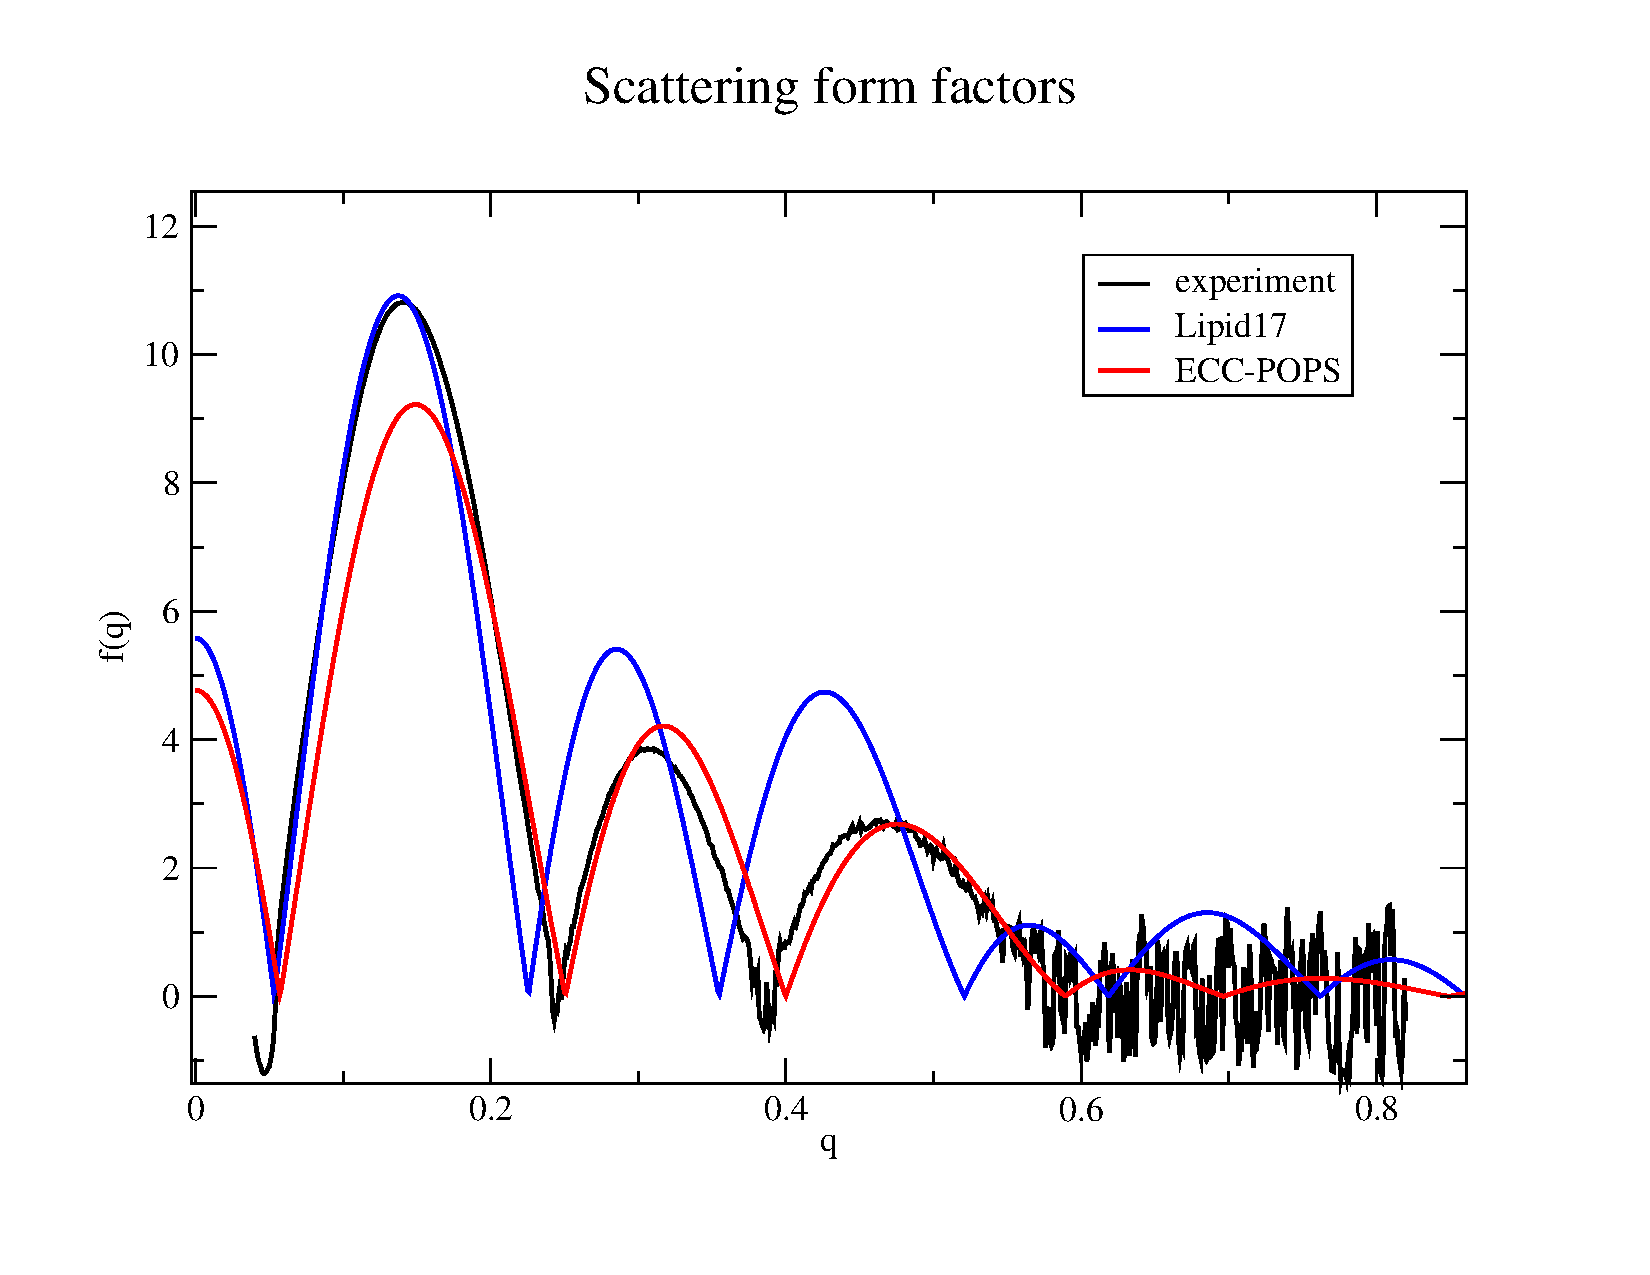
\includegraphics[width=\figwidth]{../img/ecc_pops/form-f_l17-ecc-pops-exp_compar.pdf} 
  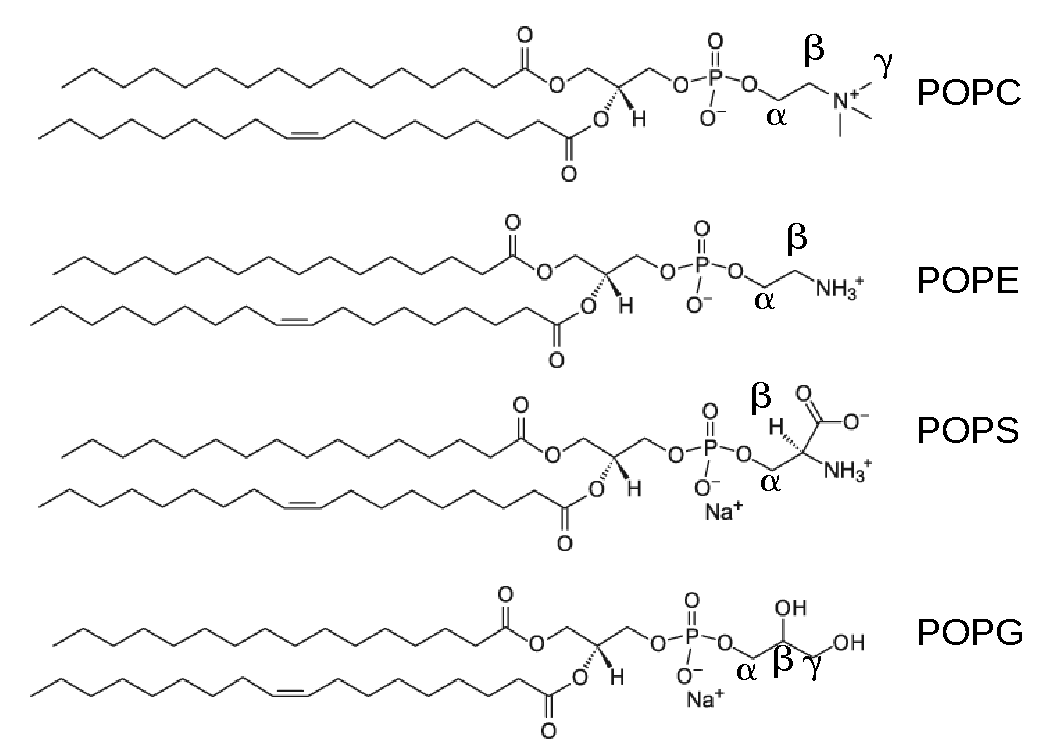
\includegraphics[width=\figwidth]{../img/ecc_pops/lipids_chemfig.pdf} 
  \caption{\label{simVSexpNOions} 
    X-ray scattering form factors from simulations with the Lipid17 \cite{lipid17-future} and 
    the ECC-POPS models compared with experiments~\cite{SDP-CHARMM36_comparison_paper_Samuli-knows} at 298~K. 
    Order parameters of POPS head group, glycerol backbone and acyl chains  
    from simulations with the Lipid17 \cite{lipid17-future} and the ECC-POPS models 
    compared with \emph{experiments at 300~K (check and change)} measured by Tiago Ferriera. 
    Open/closed symbols are used for palmitoyl/oleoyl chains of POPS. 
    The chemical structure of POPS and the labeling of the carbon segments. 
  }  
\end{figure} 
%%%%%%%%%%%%%%%%%%%%%%%%%%%%%%%%%%%%%%%%%%%%%%%%%%%%%%%%%%%%%%
 
\begin{table}[tb!] 
  \caption{Values of the area per lipid (APL) of POPC and POPS bilayers without additional ions. \label{tab:apls} 
  } 
  \begin{tabular}{l|c c} 
    \multicolumn{3}{c}{POPC} \\
    \hline 
    model          & APL (Å$^2$)   & Temperature (K) \\ 
    \hline 
    Lipid14 POPC                    & 65.1$\pm$ 0.6  &  300 \\ 
    Lipid14 POPC \citep{dickson14}  & 65.6$\pm$ 0.5  &  303 \\ 
    \hline 
    ECC-POPC                & 63.2$\pm$ 0.6  &  300       \\ 
    \hline 
    experiment (SDP model) \citep{kucerka11} & 64.3  &  303    \\ 
    \hline 
    \\
    \multicolumn{3}{c}{POPS} \\
    \hline 
    model          & APL (Å$^2$)   & Temperature (K) \\ 
    \hline 
    Lipid17 POPS              & 53.5$\pm$ 0.8  &  298 \\ 
    \hline 
    ECC-POPS                & 60.3$\pm$ 0.6  &  298       \\ 
    \hline 
    experiment (SDP model) \cite{SDP-CHARMM36_comparison_paper_Samuli-knows} & 62.3  &  298    \\ 
    \hline 
  \end{tabular} 
\end{table} 
 
 
First, we present results for bilayers in pure water. 
The ECC-POPC and Lipid14 models both reproduce the experimental X-ray scattering form factors 
of a POPC bilayer with a comparable accuracy (see Fig.~\ref{simVSexpNOions}). 
The area per lipid from the Lipid14 model is by $\approx$1Å larger than the 
experimental value in Table~\ref{tab:apls}, while the value from the ECC-POPC model 
is by $\approx$1Å smaller than the experimental one. 
The values of the area per lipid of the ECC-POPC model vary slightly 
when simulated with different water models (i.e., within the interval of 62.2--66.8 Å, see Table~S2 in SI), 
while still being close to the experimentally reported values. 
We can thus conclude that the ECC-POPC model reproduces the experimental dimensions of the POPC 
lipid bilayer with a comparable accuracy to other state-of-the-art lipid models~\citep{ollila16}. 
 
 
Similarly, the acyl chain order parameters of the ECC-POPC model, as well as those of the Lipid14 model~\citep{dickson14}, agree with the experimental values within the error bars, as presented in Fig.~\ref{simVSexpNOions}. Notably, the experimentally measured forking and small order parameter values of the $C_2$ segment in {\it sn}-2 chain are well reproduced by both models. This feature has been suggested to indicate that the carbonyl of the {\it sn}-2 chain is directed towards the water phase, in contrast to the carbonyl in the {\it sn}-1 chain, which orients more along the bilayer plane~\citep{seelig75,schindler75,gawrisch92}. 
This arrangement, which is not fully reproduced by other available lipid models~\citep{ollila16}, may be a relevant feature for the ion binding details. 
 
The order parameters of the $\alpha$ and $\beta$ carbons in the head group are slightly larger in the ECC-POPC model than in the Lipid14 model, which is apparently related to the P-N vector orienting by about 7$^{\circ}$ more toward the water phase in the former model, see Fig.~\ref{OrderParameterCHANGESsurf}. While both models perform relatively well, considering the available experimental evidence, it is not possible to decide which of the two models provides more realistic head group orientations. The ECC-POPC model gives the $\beta$ carbon order parameter value closer to experiments than the Lipid14 model, while the opposite is true for the $\alpha$ carbon. The accuracy of both models in the glycerol backbone region is comparable to other state-of-the-art lipid model available in literature \citep{botan15}, see Fig.~\ref{simVSexpNOions}. 


 
 

\chapter{Interactions of ions with phospholipid membranes}
\label{chap:results}

Biological membranes naturally exist in a weak electrolytic solution of \ce{KCl} on the intracellular side, and of \ce{NaCl} on the extracellular side. 
The biological relevance of these ions reaches from relatively simple osmotic effects to the complex processes in neural signalling. 

Calcium is an important cation in biology, 
which takes part in many signalling pathways, e.g. triggering of the release of neurotransmitter in neurons,
and processes such as regulating cardiac rythm in heart. 
The interaction of \ce{Ca^{2+}} with phospholipid membranes has recieved attention recently from both experiments and simulations \citep{melcrova16, javanainen17}.

In the previous chapter, we presented new classical MD models of phospholipids,
which account for electrionic polarization via ECC (introduced in section~\ref{section:ecc}). 
It was demonstrated that such models, termed ECC-lipids, 
meet current accuracy standards in the field 
by comparing them with NMR order parameters and X-ray diffraction data (section~\ref{section:ecc-lipids}. 

In this chapter, we will provide detailed insight into the interactions of these ions with neutral and negatively charged model membranes,
namely with a POPC bilayer and to a bilayer with a composition of 5~POPC:1~POPS. 
We employ our newly developed models of ions and phospholipids, 
ECC-ions \citep{martinek17, kohagen16, Pluharova2014} and ECC-lipids \citep{melcr18}, 
which excel any state-of-the-art model of ions or lipids. 

First, we summarize the literature knowledge on the interactions of ions with membranes in experiments and simulations.
Then we demonstrate the outstanding accuracy of the newly developed model of POPC, ECC-POPC, 
in the responses of the head group order parameters.
The simulation study with a cationic surfactant 
validates ECC-POPC as an accurate model of the lipid electrometer concept observed in NMR experimnents. 
At last, we will provide detailed insight into the binding of cations to the neutral and negatively charged bilayers. 
We put extra stress on the interactions with \ce{Ca^{2+}}, 
for which we present the first simulation results that are in \emph{quantitative} agreement with experiments. \citep{catte16, melcr18}





\section{Lipid electrometer and binding of cations to phospholipid bilayers in experiments and simulations}
\label{section:electrometer_exp_sim} 

\textbf{ Recap the main outcomes of the NMRLipids II paper \citep{catte16}. }
Then introduce/continue with how to fix it. 
Include 1-2 figures. 

\textbf{ Recap the main outcomes of the NMRLipids IV paper. }
Prepare ground for the work-in-progress POPS model. 

\textbf{Electronic polarization is required for accurate head group response to membrane-bound charge in simulation. ECC-POPC paper text follows \dots  }

\begin{figure}[tb!] 
  \centering 
  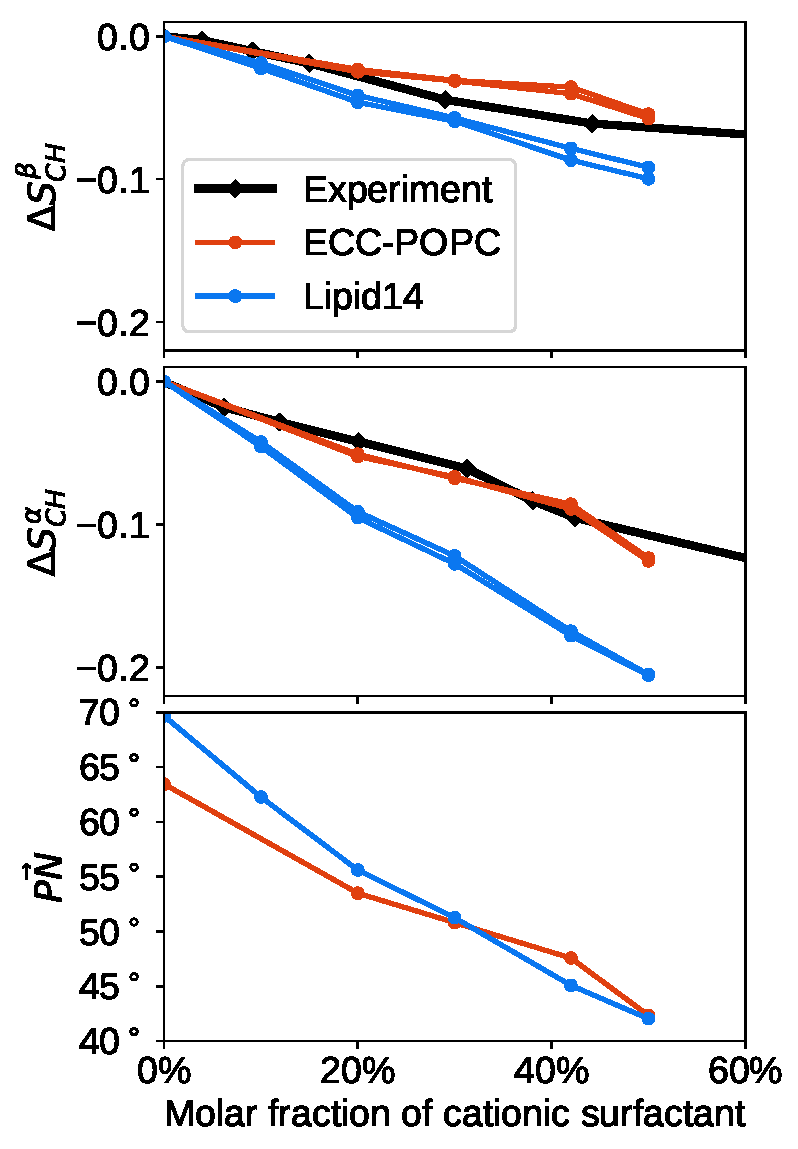
\includegraphics[width=\figwidth]{../img/ecc_popc/PN_angle_OrdPars-A-B_L14-ECCL17_q80_sig89_surf.pdf} 
  \caption{\label{OrderParameterCHANGESsurf} 
    The changes of head group order parameters and P-N vector orientation as a function of 
    a molar fraction of the cationic surfactant dihexadecyldimethylammonium in a POPC bilayer 
    from simulations and experiments \citep{scherer89} at 313 K.
  } 
\end{figure} 
 
The calibration of the response of the lipid electrometer to the amount of bound charge 
is measured for mixtures of POPC with monovalent cationic surfactants \citep{scherer89}.
In this work, we have chosen dihexadecyldimethylammonium. 
The amount of bound charge per PC 
in such systems is simply given by the molar fraction of the cationic surfactants, 
as essentially all of the surfactants locate to the lipid bilayers 
due to the two long hydrophobic tails.
The NMR measurements of such systems  
can be used to validate the sensitivity of lipid headgroup order parameters 
(i.e. the coefficient $m_i$ from Equation~\ref{OPchangeEQ}) 
to the amount of bound charge in simulations \citep{scherer89}.

The changes of the headgroup order parameters with an increasing amount of 
the cationic surfactant from simulations and experiments~\citep{scherer89} are shown in Fig.~\ref{OrderParameterCHANGESsurf}.
In line with Equation~\ref{OPchangeEQ},
we observe in both simulations and experiments approximately a linear decrease of the head group order parameters $\alpha$ and $\beta$.
The slope of the response from the simulation with ECC-POPC model 
is in a very good agreement with the experiments for the $\alpha$ segment, 
while being slightly underestimated for the $\beta$ segment at higher concentrations.
In addition to the order parameters, we also show the change of the P-N vector, 
which is plotted as the angle between the connector of the phosphorus and nitrogen atoms and the membrane normal. 
Again, there is a linear dependence on the amount of surface charge
suggesting a possible relation between the order parameters and the P-N vector mean orientation. 
\todo{Provide the relation explicitly somewhere? -- Yes.}

For a direct comparison, we also provide results from simulations with the Lipid14 model. 
It is already noted in our publication \citep{melcr18} that
the response of the head group order parameteres to the bound charge 
is overestimated in this model yielding a too steep slope of the response to the increasing amount of the cationic surfactant. 
It is clear from the above discourse that accounting for electronic polarization is crucial for an accurate response of the lipid electrometer in simulation. 
After reproducing the concept of electrometer with a known amount of bound surface charge,
the ECC-POPC model will be employed in the study of interactions with aquaeous ions, namely \ce{K}, \ce{Na+} and \ce{Ca^{2+}}. 









\section{Interactions of neutral and negatively charged phospholipid membranes with K$^+$, Na$^+$}

\begin{figure}[htb!] 
  \centering 
  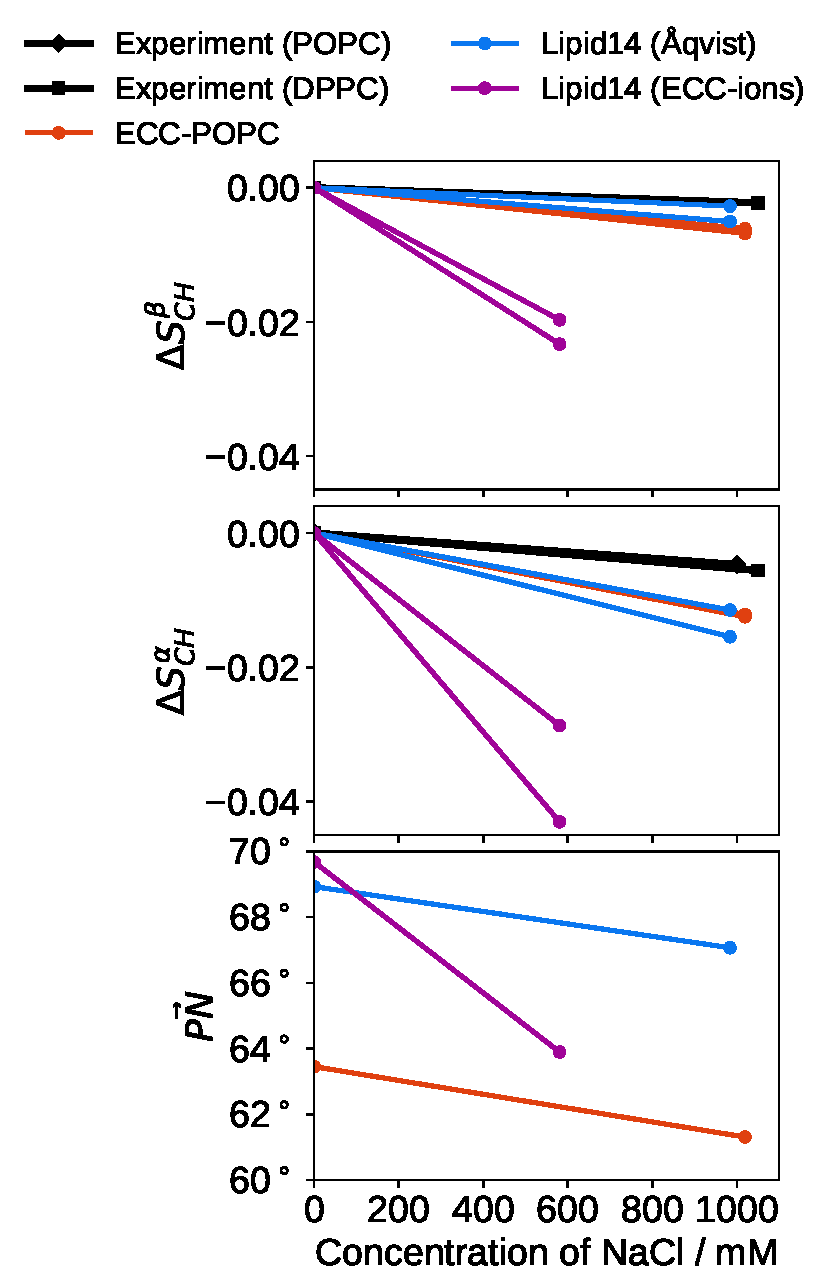
\includegraphics[height=10 cm]{../img/ecc_popc/OrdPars-A-B-PNvec_L14-ECC-lipids_NaCl.pdf}
  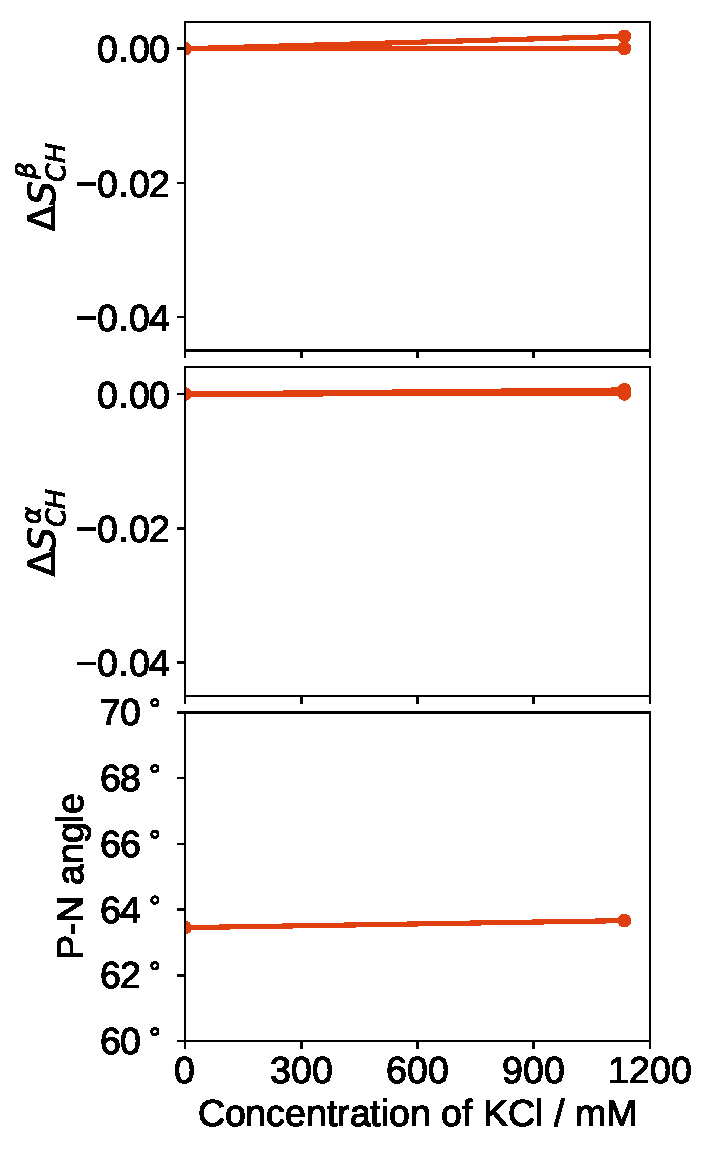
\includegraphics[height= 9 cm]{../img/ecc_popc/OrdPars-A-B-PNvec_L14-ECC-lipids_KCl.pdf}
  \caption{\label{fig:delta_ordPar_NaCl} 
    Changes of the head group order parameters of a POPC bilayer as a function of \ce{NaCl} (left) and \ce{KCl} (right) concentration 
    in bulk ($C_{ion}$) from simulations with different force fields at 313 K together with  
    experimental data for DPPC (323\,K) \citep{akutsu81} and POPC (313\,K) \citep{altenbach84}. 
    Simulation data with Lipid14 and Åqvist ion parameters at 298 K are taken directly from 
    Refs.~\citep{lipid14POPC0mMNaClfiles,lipid14POPC1000mMNaClfiles}. 
  } 
\end{figure} 
 

 
\begin{figure}[tbp!] 
  \centering 
  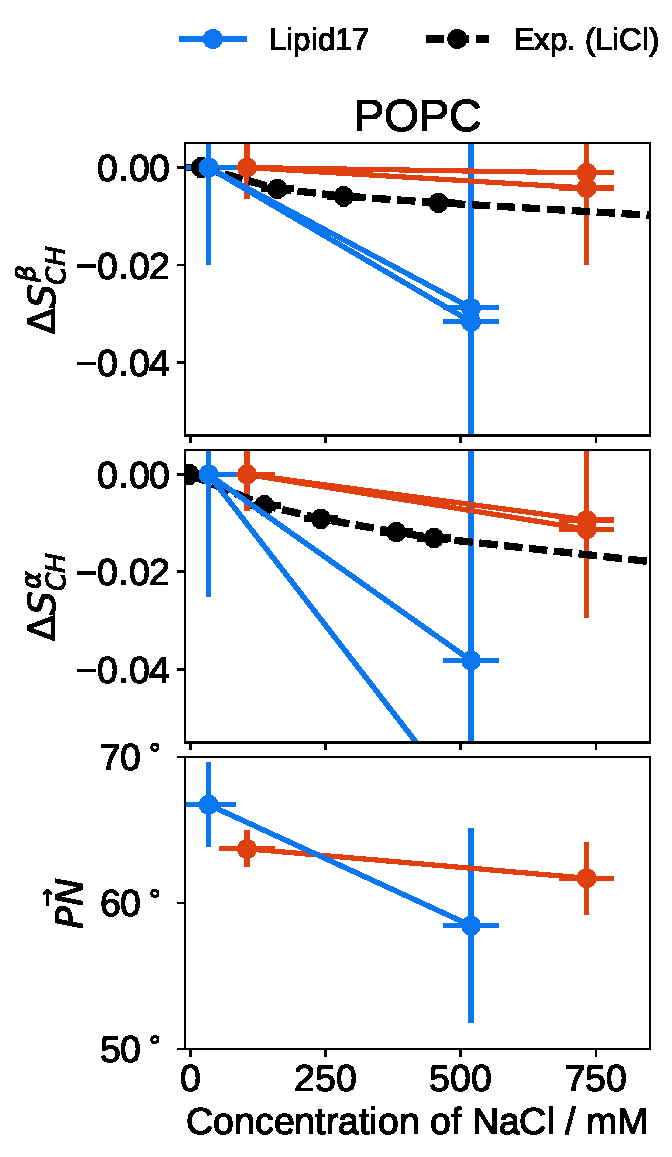
\includegraphics[width=\figwidthsmall]{../img/ecc_pops/order_parameters_changes_ecc-lip_L14_A-B-PN-COO_POPC_nacl.pdf} 
  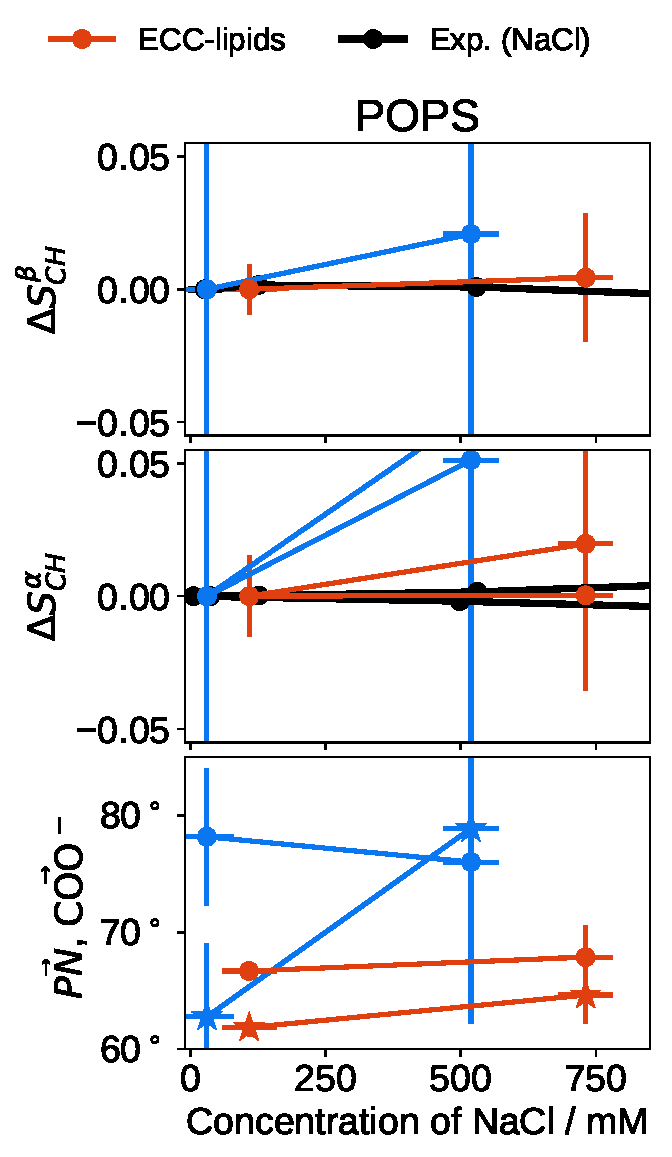
\includegraphics[width=\figwidthsmall]{../img/ecc_pops/order_parameters_changes_ecc-lip_L14_A-B-PN-COO_POPS_nacl.pdf} 
\todo{Add LiCl resp. NaCl labels to experiments in legend. Remove the legend for ECC-lipids in one of the plots -- they are side by side and hence it is duplicate.}
  \caption{\label{fig:delta_ordPar_NaCl} 
    Changes of the head group order parameters $\alpha$, $\beta$ and the orientations of the carboxylate group and the P-N vector  
    of POPC (left) and POPS (right) phospholipids in a POPC:POPS 5:1 bilayer as a function of \ce{NaCl} concentration 
    in bulk ($C_{ion}$) from simulations with different force fields at 298 K.
    Because data with \ce{NaCl} are not available for POPC, 
    we show experimental data for \ce{LiCl} (dashed line, left) \citep{roux90}
    as an upper bound for the magnitude of the response to \ce{NaCl}, 
    which has a lower affinity to phospholipid bilayers compared to \ce{LiCl}. 
    The orientation of the \ce{COO^-} group is defined as 
    the connector from the $\beta$ carbon to the carbon in \ce{COO^-} (stars, bottom right). 
  } 
\end{figure} 



\begin{figure}[tbp!] 
  \centering 
  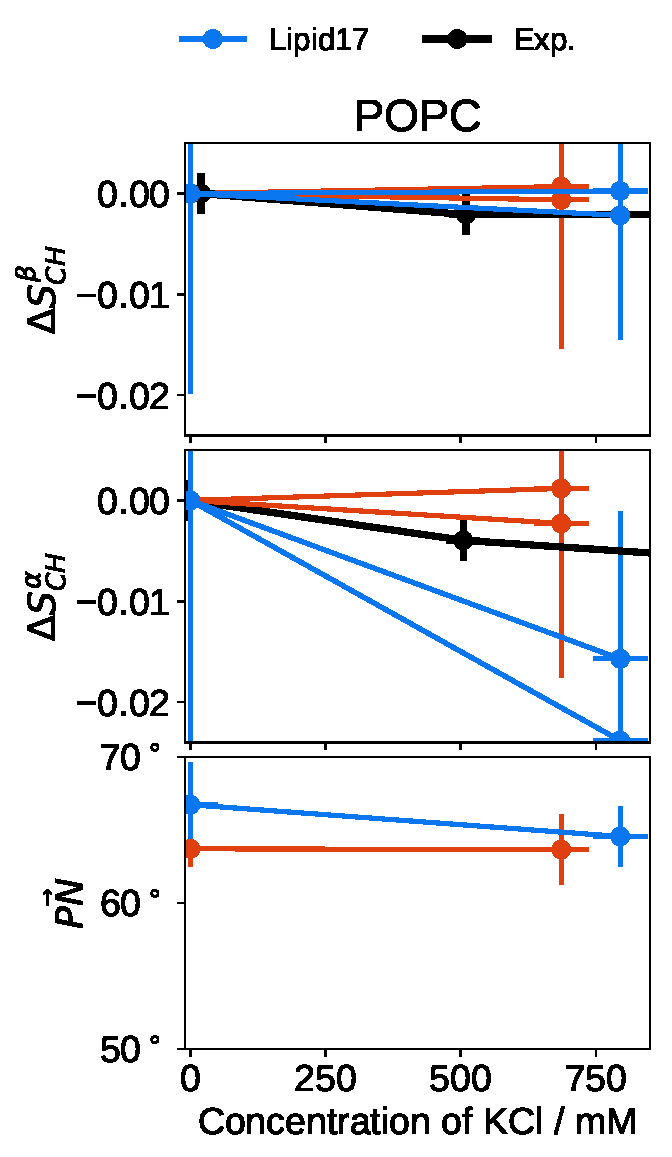
\includegraphics[width=\figwidthsmall]{../img/ecc_pops/order_parameters_changes_ecc-lip_L14_A-B-PN-COO_POPC_kcl.pdf} 
  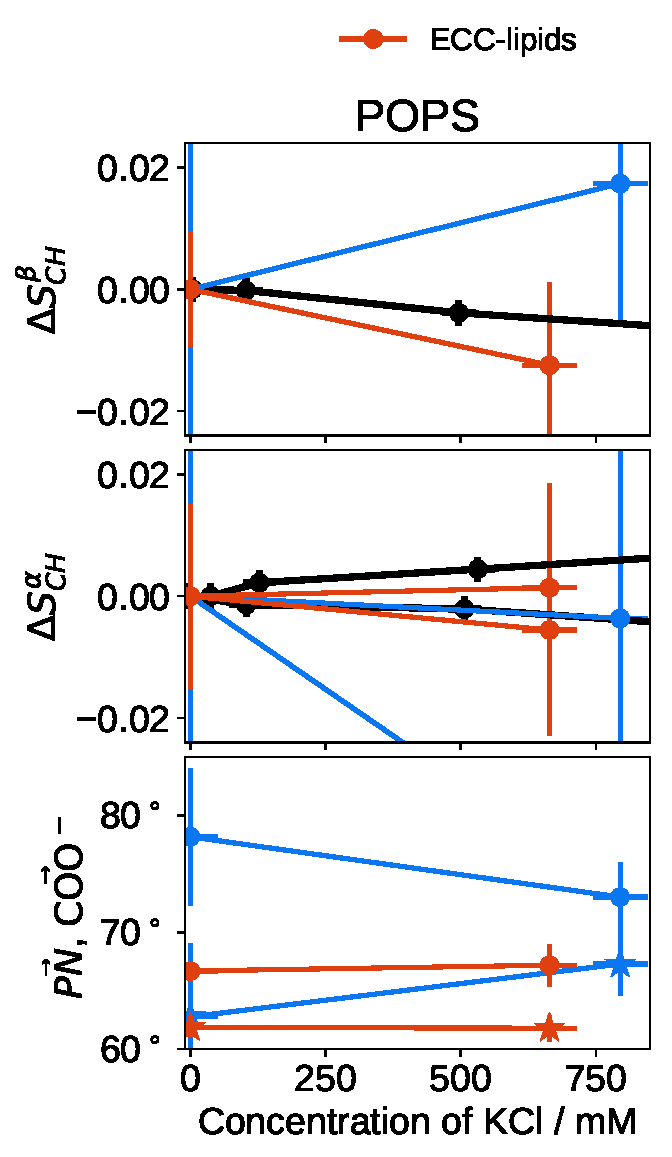
\includegraphics[width=\figwidthsmall]{../img/ecc_pops/order_parameters_changes_ecc-lip_L14_A-B-PN-COO_POPS_kcl.pdf} 
\todo{Remove the extra legend.}
  \caption{\label{fig:delta_ordPar_KCl} 
    Changes of the head group order parameters $\alpha$, $\beta$ and the orientations of the carboxylate group and the P-N vector  
    of POPC (left) and POPS (right) phospholipids in a POPC:POPS 5:1 bilayer as a function of \ce{KCl} concentration 
    in bulk ($C_{ion}$) from simulations with different force fields and experiments at 298 K. \citep{roux90}
    The orientation of the \ce{COO^-} group is defined as 
    the connector from the $\beta$ carbon to the carbon in \ce{COO^-} (stars, bottom right). 
  } 
\end{figure} 
 


\todo{Rewrite this whole section.}

 
Changes of the lipid bilayer head group order parameters extracted from simulations and 
experiments \citep{akutsu81, altenbach84} are shown in Figs.~\ref{fig:delta_ordPar_NaCl} 
and~\ref{fig:delta_ordPar_CaCl} as functions of NaCl or CaCl$_2$ concentrations. 
As seen in Fig.~\ref{OrderParameterCHANGESsurf}, the order parameters decrease 
proportionally to the amount of the bound positive charge. 
These results can be thus used to compare the ion binding affinities to lipid bilayers between 
simulations and experiments using the electrometer concept~\citep{seelig87, catte16}. 
 
The experimentally measured small order parameter 
changes with NaCl (Fig.~\ref{fig:delta_ordPar_NaCl})  
are reproduced by the Lipid14 model simulated with Åqvist ions. 
However, the same combination of models overestimates the order parameter changes with CaCl$_2$ (Fig.~\ref{fig:delta_ordPar_CaCl}). 
Replacing Åqvist ions with ion parameters by Dang et al.~\citep{smith94, chang1999, dang2006} 
or ECC-ions~\citep{martinek17, kohagen16, Pluharova2014} did not improve 
the results~(Figs.~\ref{fig:delta_ordPar_NaCl} and \ref{fig:delta_ordPar_CaCl}). 
In line with the previous work \citep{catte16}, the results suggest that improvements 
in the lipid parameters are required to correctly describe the binding of cations to phospholipid bilayers. 
 

\begin{figure}[tbp!] 
  \centering 
  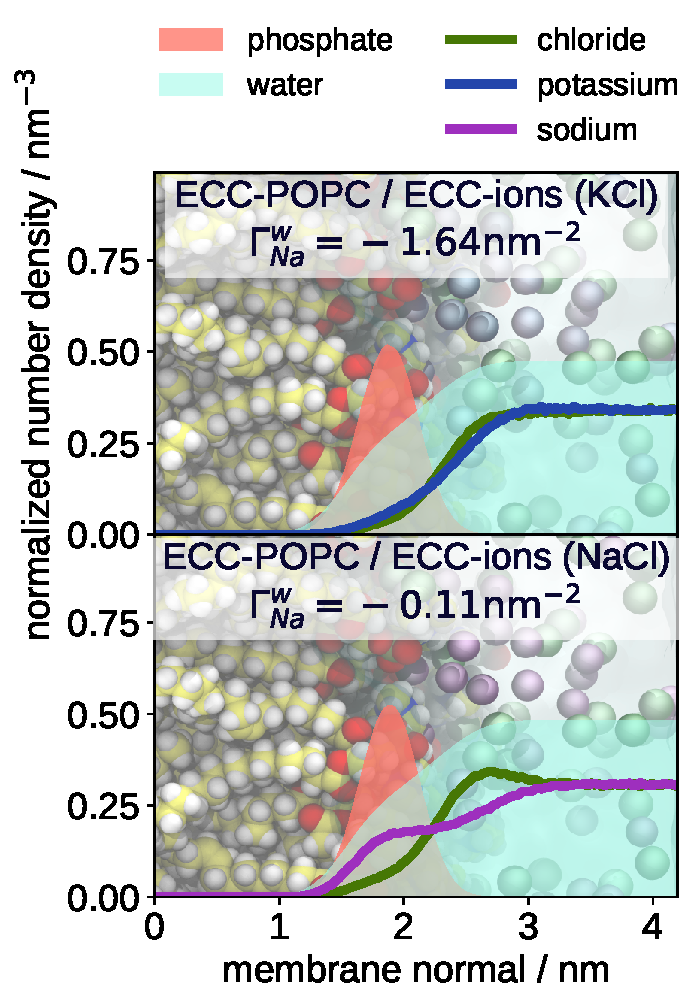
\includegraphics[width=\figwidth]{../img/ecc_popc/density_profiles_ca_cl_wat_phos_models-compar_5-7_NaCl-KCl.pdf}
  \caption{\label{fig:nacl-dens} 
    Number density profiles of \ce{K^{+}}, \ce{Na^{+}} and \ce{Cl^-} along membrane normal axis 
    from the simulations with ECC-lipids and ECC-ions with neutral POPC bilayer.  
    In order to visualize the density profiles with a scale comparable to the profile of \ce{Ca^{2+}} in Fig.~\ref{fig:cacl-dens},  
    the density profiles of~\ce{Cl^-}, \ce{K^+} and \ce{Na^+} ions are divided by 2, and 
    the density profiles of phosphate groups and water are divided by 5 and 200, respectively.  
    The simulation with \ce{NaCl} has $C_{ion}'$=1000~mM, 
    the simulation with \ce{KCl}  has $C_{ion}'$=1100~mM. 
    } 
\end{figure} 


\begin{figure}[tbp!] 
  \centering 
  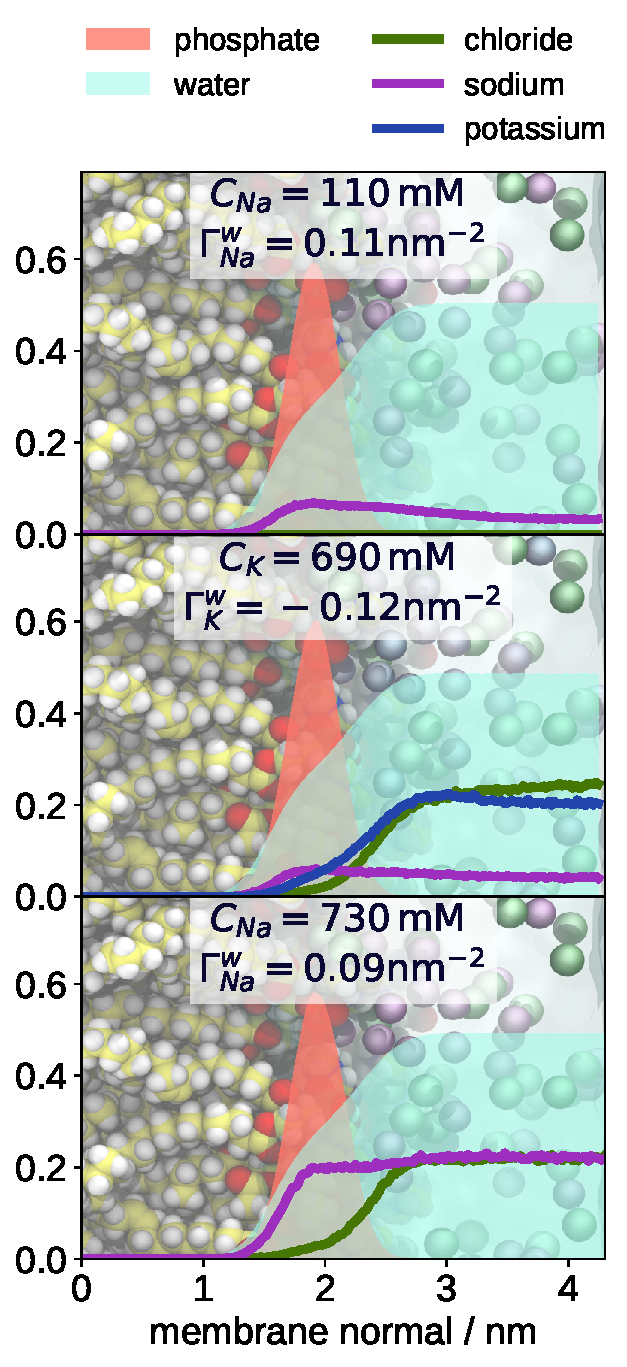
\includegraphics[width=\figwidth]{../img/ecc_pops/density_profiles_na_k_cl_wat_phos_models-compar_4-6_NaCl-and-KCl-series.pdf}
\todo{Change the labels in the figure so that the $C_{ion}$ tells explicitly \emph{which} ion.}
  \caption{\label{fig:nacl-dens_PCPS} 
    Number density profiles of \ce{K^{+}}, \ce{Na^{+}} and \ce{Cl^-} along membrane normal axis 
    for the negatively charged membrane with the composition of 5\,PC:1\,PS. 
    The top profile shows the simulation without any additional salt concentration, i.e. only with \ce{Na^+} counterions. 
    The middle profile shows the simulation with an additional \ce{KCl} concentration and \ce{Na^+} counterions. 
    The bottom profile shows the simulation with an additional \ce{NaCl} concentration and \ce{Na^+} counterions, which are not distinguished from the added salt. 
    In order to visualize the density profiles with a scale comparable to the profile of \ce{Ca^{2+}} in Fig.~\ref{fig:cacl-dens},  
    the density profiles of~\ce{Cl^-}, \ce{K^+} and \ce{Na^+} ions are divided by 2, and 
    the density profiles of phosphate groups and water are divided by 5 and 200, respectively.  
    } 
\end{figure} 



The results from simulations combining the ECC-POPC with the ECC-ion models \citep{martinek17, kohagen16, Pluharova2014} exhibit a significantly improved behavior of the POPC head group order parameters as a function of NaCl or CaCl$_2$ concentrations, see Fig.~\ref{fig:delta_ordPar_NaCl} and Fig.~\ref{fig:delta_ordPar_CaCl}. Considering that we are also able to reproduce the experimental response in systems with known charge density (see above section \ref{section:boundCHARGE}), we conclude that our ECC model correctly reproduces the binding affinities of Na$^{+}$ and Ca$^{2+}$ ions to the POPC lipid bilayer. Furthermore, while the response of the glycerol backbone $g_3$ order parameter to CaCl$_2$ was significantly overestimated in the original Lipid14 model, the ECC-POPC model provides an improved agreement with experiment, as seen in Fig.~\ref{fig:delta_ordPar_CaCl}. 
Also the changes of the P-N vector angle are too pronounced for the Lipid14 model, 
for which the largest tilting toward water phase induced by a $780\,\mathrm{mM}$ 
CaCl$_2$ concentration is approximately 17$^{\circ}$. The corresponding value 
for the ECC-POPC simulation is only 6$^{\circ}$ ($820\,\mathrm{mM}$ CaCl$_2$).  

% on the binding affinity using surface excess:
Interestingly, the calculated relative surface excess of \ce{NaCl} at $1\,\mathrm{M}$ concentration (ECC-ions~\citep{Pluharova2014}) using our ECC-POPC model is not only quantitatively but also qualitatively different from \ce{CaCl2} having actually a negative value of $\Gamma_{Na}^{water} = -0.11 \pm 0.01) \rm{nm}^{-2}$ (Fig.~\ref{fig:nacl-dens}. This  
means that on average water molecules are preferred to sodium and chloride ions at the membrane-water interface.   
This is in contradiction with most of the available lipid force fields, which predict a positive surface excess of sodium at PC lipid bilayers \citep{catte16}. 
 
Even though \ce{Na+} ions do not bind strongly to a POPC bilayer, they still interact mostly with its oxygen moieties. 
The results from a simulation at a $1\,$M \ce{NaCl} concentration show that 55\% of \ce{Na+} ions at the bilayer interact with phosphate oxygens of POPC only and 20\% with carbonyl oxygens only, with the remaining 25\%, is interacting with both negatively charged groups. 
Sodium ions, which do not exhibit any appreciable affinity for the bilayer, also interact primarily with phosphate oxygens of the POPC, but in contrast to calcium, the interactions purely with carbonyls are also significant. 
 
The probabilities of different complexes formed by \ce{Na+} ions and POPC 
analyzed from the simulation with the ECC-POPC model at $1\,$M concentration of NaCl are also  
shown in Fig.~\ref{fig:cacl_complexes}. In contrast to calcium, the 
probability is largest (67\%) for 1:1 complex, significantly smaller (29\%) 
for 1:2 complexes and very small (4\%) for 1:3 of \ce{Na+}:POPC complexes. 
 
Note that the exchange of \ce{Na+} ions at the POPC membrane 
is yet another order of magnitude faster, with 90\% of the residence times smaller than~1~ns and the longest residence time being~6~ns. 
 
Finally, the ion binding affinities for the ECC-POPC model with different water models are compared in SI. In general, the performance of ECC-POPC with any of the tested water models is better than that of the original Lipid14 model, with the order parameter changes being slightly overestimated with the four-site water models and with TIP3P model. 
 





 
 


\section{Interactions of neutral and negatively charged phospholipid membranes with \ce{Ca^{2+}}}

\todo{Rewrite this whole section.}


\begin{figure}[htb!] 
  \centering 
  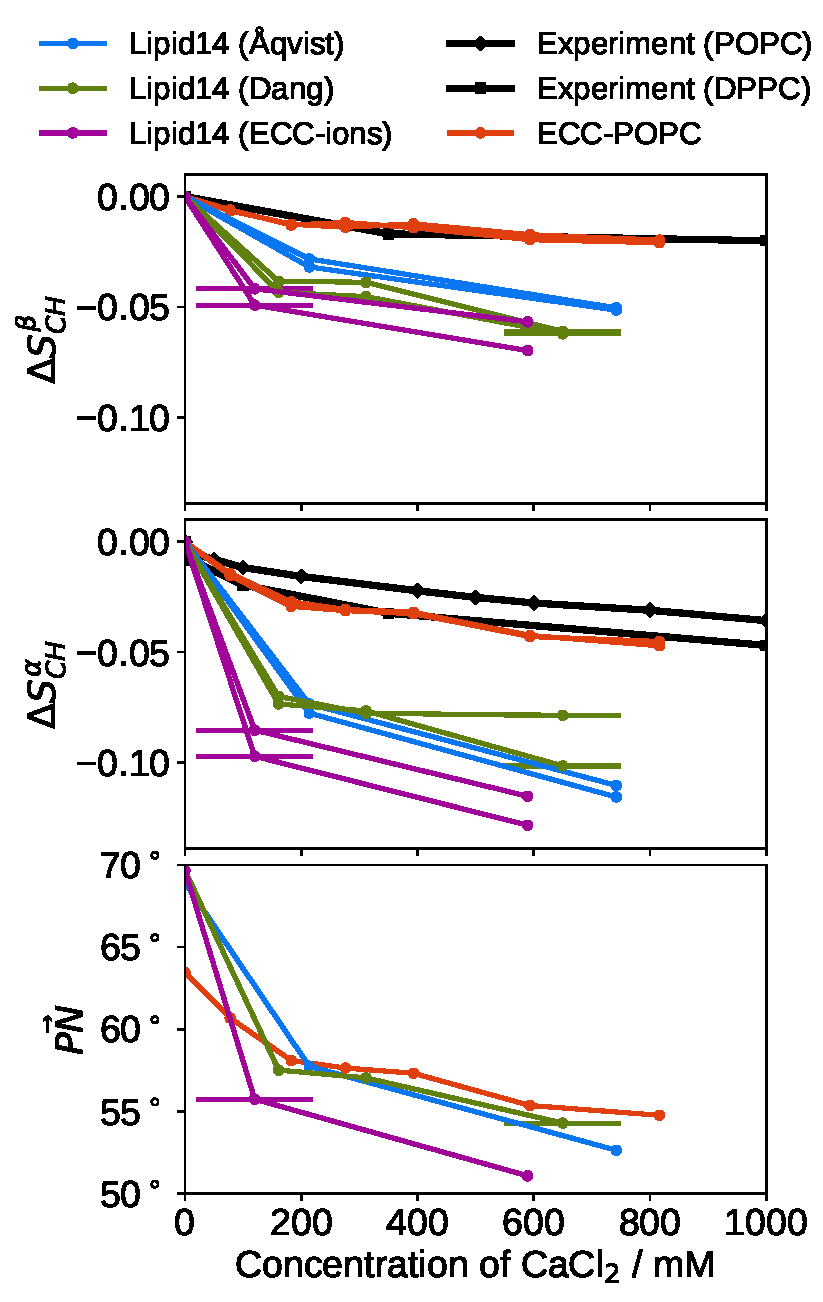
\includegraphics[width=\figwidth]{../img/ecc_popc/OrdPars-A-B-PNvec_L14-ECC-lipids_CaCl.pdf}
  \caption{\label{fig:delta_ordPar_CaCl} 
    Changes of the head group order parameters and P-N vector orientation of a POPC bilayer  
    as a function of the CaCl$_2$ concentration in bulk ($C_{ion}$) 
    from simulations at 313 K together with experimental data  
    (DPPC (323\,K) \citep{akutsu81} and POPC (313\,K) \citep{altenbach84}).  
    The error estimate for bulk concentrations is approximately 10\,mM. 
    The order of magnitude larger error in the
    simulation with Lipid14 and ECC-ions is due to unconverged bulk densities  (shown if Fig.~\ref{fig:cacl-dens}) limited by
    the simulation box.  
    Simulation data with Lipid14 and Åqvist ion parameters at 298 K are taken directly from 
    Refs.~\citep{lipid14POPC0mMNaClfiles,lipid14POPC350mMCaClfiles,lipid14POPC350mMCaClfilesNC}. 
  } 
\end{figure} 


\begin{figure}[htb!] 
  \centering 
  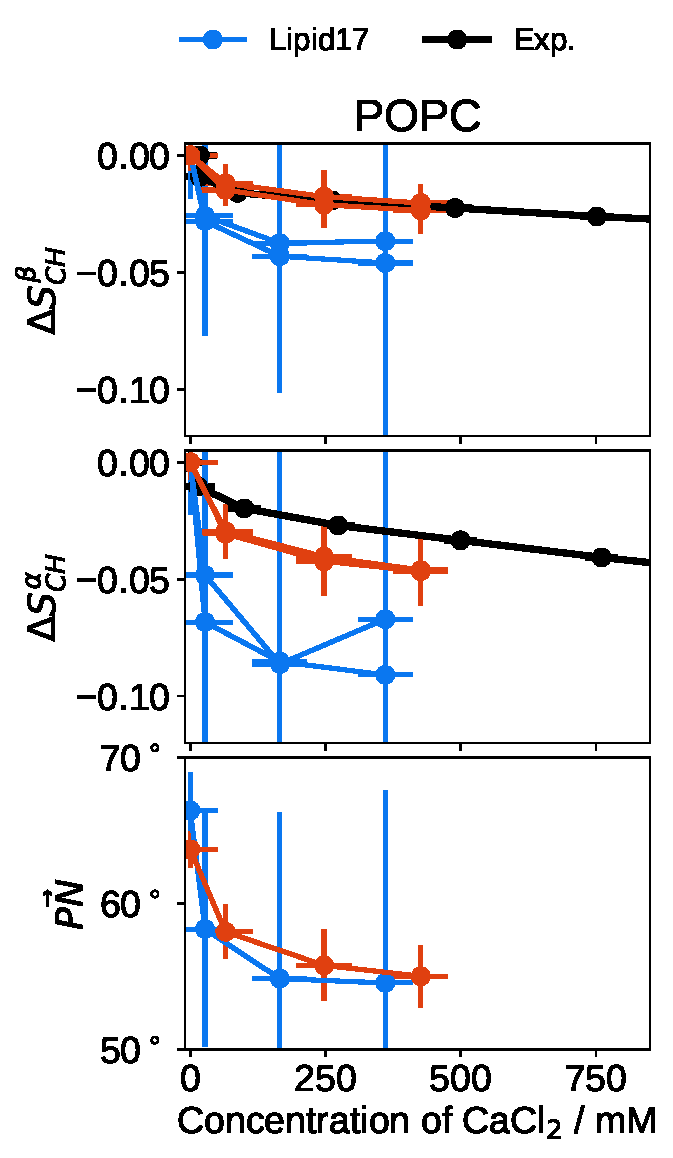
\includegraphics[width=\figwidthsmall]{../img/ecc_pops/order_parameters_changes_ecc-lip_L14_A-B-PN-COO_POPC_cacl.pdf} 
  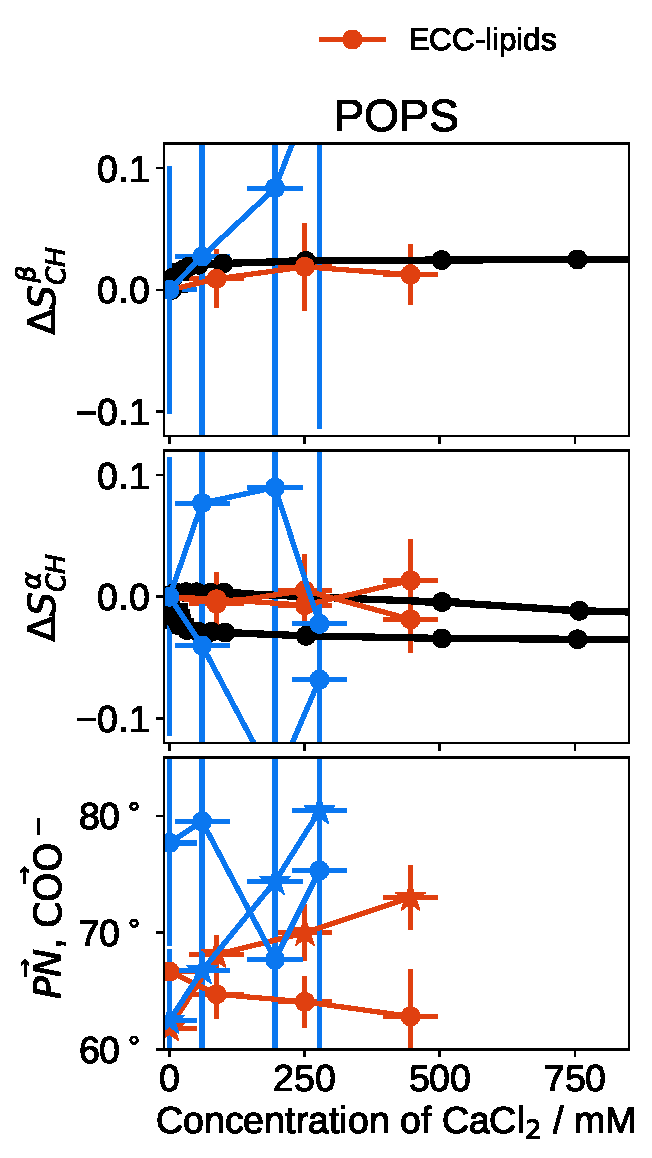
\includegraphics[width=\figwidthsmall]{../img/ecc_pops/order_parameters_changes_ecc-lip_L14_A-B-PN-COO_POPS_cacl.pdf} 
\todo{Remove the extra label}
  \caption{\label{fig:delta_ordPar_CaCl_PCPS} 
    Changes of the head group order parameters $\alpha$, $\beta$ and the orientations of the carboxylate group and the P-N vector  
    of POPC (left) and POPS (right) phospholipids in a POPC:POPS 5:1 bilayer as a function of \ce{CaCl2} concentration 
    in bulk ($C_{ion}$) from simulations with different force fields and experiments at 298 K. \citep{roux90}
    The orientation of the \ce{COO^-} group is defined as 
    the connector from the $\beta$ carbon to the carbon in \ce{COO^-} (stars, bottom right). 
  } 
\end{figure} 



Changes of the lipid bilayer head group order parameters extracted from simulations and 
experiments \citep{akutsu81, altenbach84} are shown in Fig.~\ref{fig:delta_ordPar_CaCl} 
as a function of CaCl$_2$ concentration. 
As seen in Fig.~\ref{OrderParameterCHANGESsurf}, the order parameters decrease 
proportionally to the amount of the bound positive charge. 
These results can be thus used to compare the ion binding affinities to lipid bilayers between 
simulations and experiments using the electrometer concept~\citep{seelig87, catte16}. 

The results from simulations combining the ECC-POPC with the ECC-ion models \citep{martinek17, kohagen16, Pluharova2014} exhibit a significantly improved behavior of the POPC head group order parameters as a function of NaCl or CaCl$_2$ concentrations, see Fig.~\ref{fig:delta_ordPar_NaCl} and Fig.~\ref{fig:delta_ordPar_CaCl}. Considering that we are also able to reproduce the experimental response in systems with known charge density (see above section \ref{section:boundCHARGE}), we conclude that our ECC model correctly reproduces the binding affinities of Na$^{+}$ and Ca$^{2+}$ ions to the POPC lipid bilayer. Furthermore, while the response of the glycerol backbone $g_3$ order parameter to CaCl$_2$ was significantly overestimated in the original Lipid14 model, the ECC-POPC model provides an improved agreement with experiment, as seen in Fig.~\ref{fig:delta_ordPar_CaCl}. 
Also the changes of the P-N vector angle are too pronounced for the Lipid14 model, 
for which the largest tilting toward water phase induced by a $780\,\mathrm{mM}$ 
CaCl$_2$ concentration is approximately 17$^{\circ}$. The corresponding value 
for the ECC-POPC simulation is only 6$^{\circ}$ ($820\,\mathrm{mM}$ CaCl$_2$).  

Within the Lipid14 model, the overestimated changes in the lipid headgroup order parameter of POPC  as functions of the CaCl$_2$ concentration arise both from the overestimated binding affinity and the excessive sensitivity of the headgroup tilt to the bound positive charge. It is plausible to assume that the same applies to the other lipid models tested in a previous study~\citep{catte16}, which underlines the importance of validation of the lipid headgroup order parameter response to the bound charge.  

 
Binding affinities of Ca$^{2+}$ ions to a POPC bilayer in different simulation models were quantified by calculating the relative surface excess of calcium with respect to water molecules, $\Gamma_{\rm ion}^{\rm water}$, from Eq.~\ref{surfexcess}. 
The values of $\Gamma_{\rm ion}^{\rm water}$ 
from different simulations with the same molar concetration of cations with respect 
to water ($C_{ion}'$=350mM) are shown in Table~\ref{tab:binding}. 
As expected from the changes of the lipid headgroup order parameters in Fig.~ \ref{fig:delta_ordPar_CaCl}, the relative surface excess of calcium, $\Gamma_{\rm Ca}^{\rm water}$ = 0.06~nm$^{-2}$, is significantly smaller for the ECC-POPC model than for the other models, 0.13--0.35~nm$^{-2}$. 
 


\begin{figure}[htbp!] 
  \centering 
  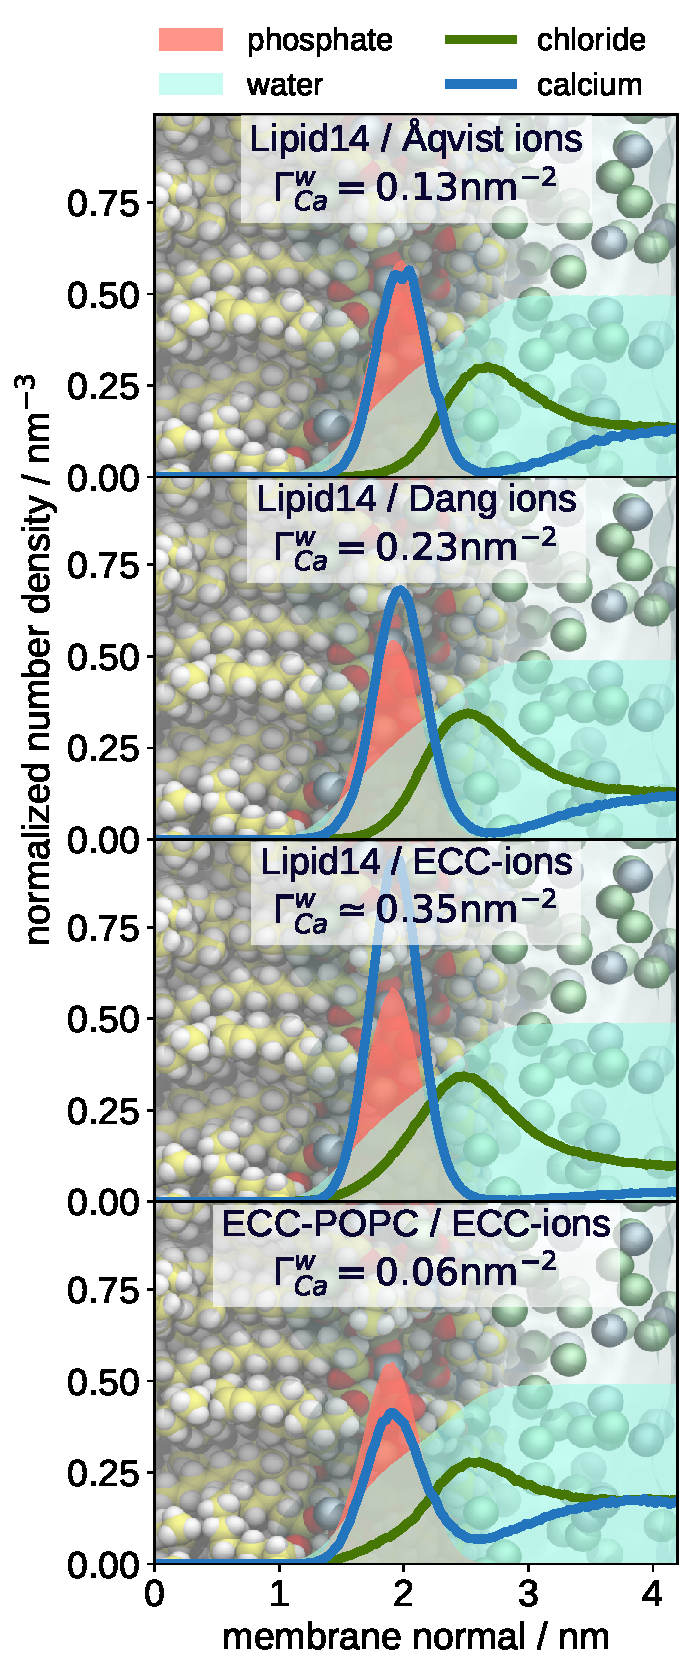
\includegraphics[width=\figwidth]{../img/ecc_popc/density_profiles_ca_cl_wat_phos_models-compar_1-4.pdf} 
  \caption{\label{fig:cacl-dens} 
    Number density profiles of \ce{Ca^{2+}}, \ce{Na^{+}} and \ce{Cl^-} along membrane normal starting at the centre of the bilayer 
    for different force fields. 
    In order to visualize the density profiles with a scale comparable to the profile of \ce{Ca^{2+}},  
    the density profiles of~\ce{Cl^-} ions are divided by 2, and 
    the density profiles of phosphate groups and water are divided by 5 and 200, respectively.  
    All simulations with \ce{CaCl2} shown here have the same molar concentration of ions in water ($C_{ion}'$=350~mM). 
    } 
\end{figure} 


\begin{figure}[htbp!] 
  \centering 
  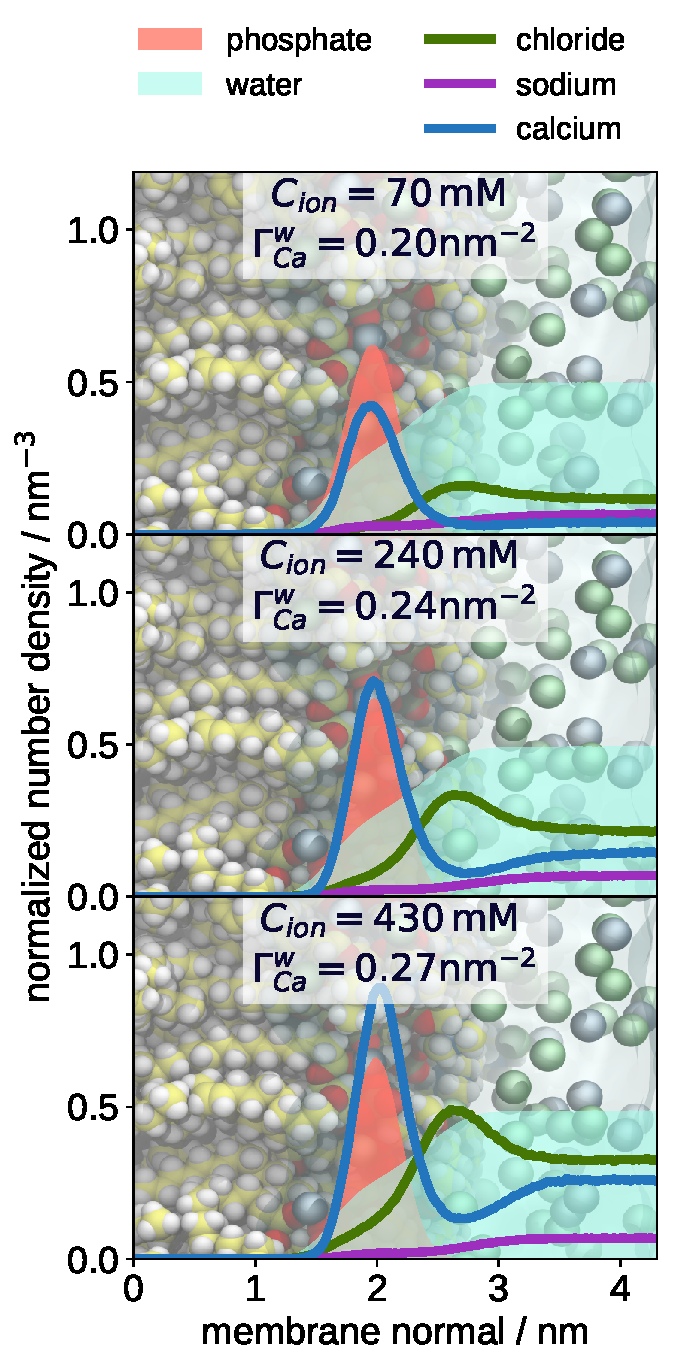
\includegraphics[width=\figwidth]{../img/ecc_pops/density_profiles_ca_na_cl_wat_phos_models-compar_1-3_CaCl2-series.pdf}
\todo{Change $C_{ion}$ to explicitly tell, which cation (\ce{Ca^{2+}}).}
  \caption{\label{fig:cacl-dens_PCPS} 
    Number density profiles of \ce{Ca^{2+}}, \ce{Na^{+}} and \ce{Cl^-} along membrane normal starting at the centre of the bilayer 
    for the negatively charged membrane of a composition 5\,PC:1\,PS
    at various bulk concentrations of \ce{CaCl2} from simulations. 
    All profiles contain \ce{Na^+} counterions and an additional concentration of \ce{CaCl2}. 
    In order to visualize the density profiles with a scale comparable to the profile of \ce{Ca^{2+}},  
    the density profiles of~\ce{Cl^-} ions are divided by 2, and 
    the density profiles of phosphate groups and water are divided by 5 and 200, respectively.  
    } 
\end{figure} 
 


\begin{table}[tb!] 
\centering
  \caption{Bulk concentrations, $C _{ion}$, and molar fractions, $C' _{ion}$, of Ca$^{2+}$;
           relative surface excess of calcium with respect to water ($\Gamma_{Ca}^{\rm water}$); 
           and percentages of the population 
           of bound Ca$^{2+}$ to various moieties 
           in a neutral membrane composed of POPC
           and in a negatively charged membrane with a compostion 5\,PC:1\,PS.
           \label{tab:binding}} 
  \begin{tabular}{ l | c c } 
	                     &  5\,POPC:1\,POPS &  POPC   \\
	\hline
	$C _{ion}\,/\,\mathrm{mM}$  &  $240\pm 10 $  &  $280\pm 10 $  \\
	$C'_{ion}\,/\,\mathrm{mM}$  &  $400\pm 10 $  &  $350\pm 10 $  \\
	$\Gamma_{Ca}^{\rm water}\, / \,\mathrm{nm}^{-2}$  &  $0.24 \pm 0.01 $  &  $0.06 \pm 0.01 $  \\
	\hline
                             &  \multicolumn{2}{c}{ } \\
        interacting moiety   &  \multicolumn{2}{c}{percentage of bound \ce{Ca^{2+}} } \\
	\hline
	     PC              &   57   &  100   \\
	     PO$_4$    in PC &   40   &   67   \\
	     carbonyls in PC &   ~1   &   ~1   \\
	\hline
	     PS              &    7   &        \\ 
	     PO$_4$  in PS   &    2   &        \\
	     COO$^-$ in PS   &    4   &        \\
	     carbonyls in PS &   ~1   &        \\
	\hline
	both PC and PS       &   36   &        \\
  \end{tabular} 
\end{table} 



\begin{figure}[tb!] 
  \centering 
  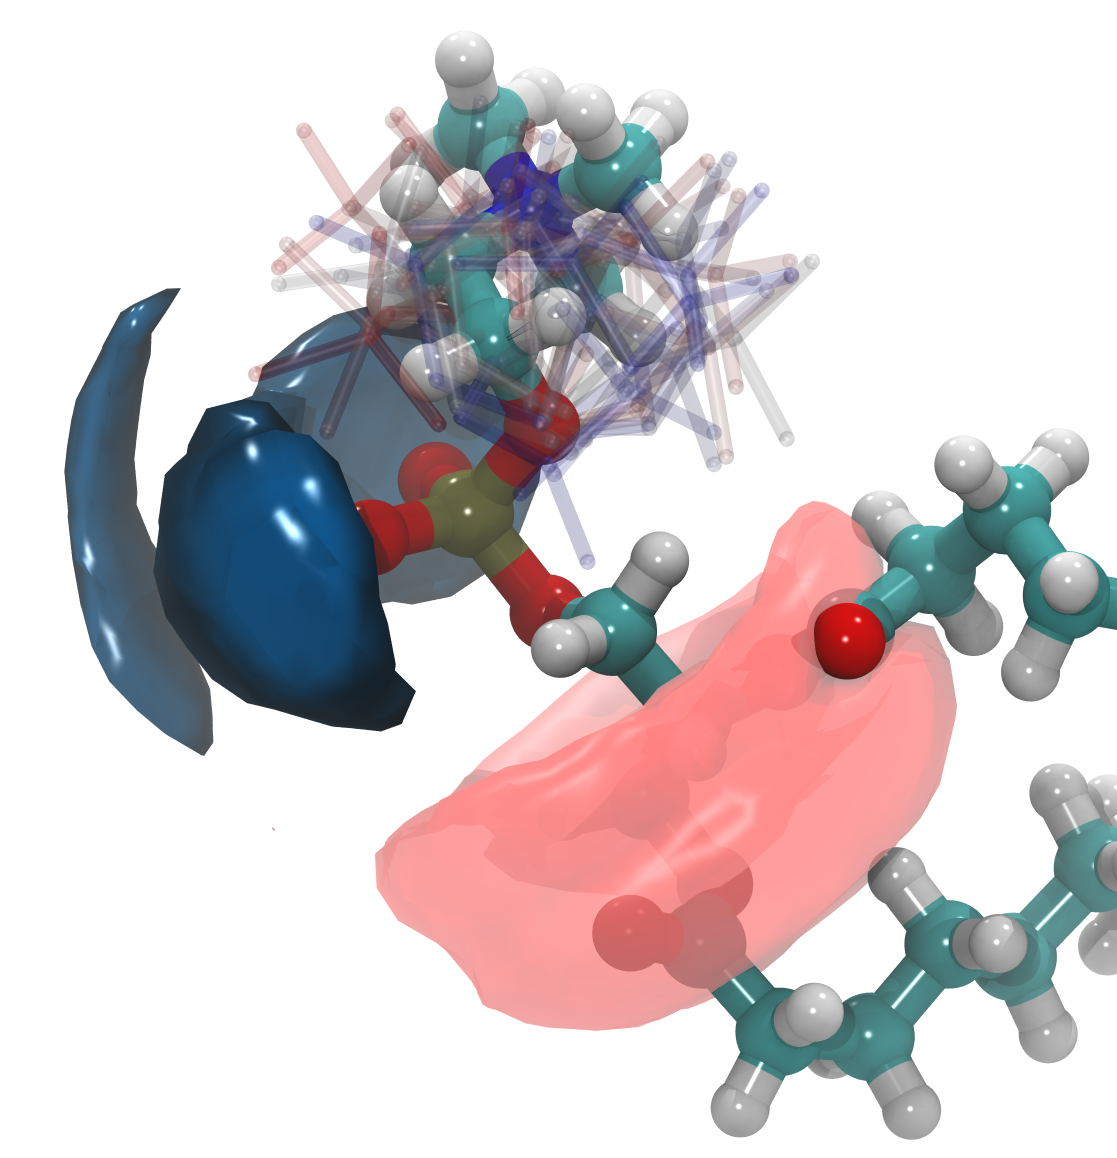
\includegraphics[width=\figwidth]{../img/ecc_popc/isocontours_r37_ca_O-carb.png} 
  \caption{\label{fig:volmaps} 
    Isocontours of spatial number density of \ce{Ca^{2+}} (dark blue, 0.001~Å$^{-3}$) 
    and POPC carbonyl oxygen atoms (light semi-transparent red, 0.008~Å$^{-3}$, all POPC lipids contribute). 
    Calcium cations localize mostly around phosphate oxygens (oxygens red, phosphorus bronze).
    Interactions with carbonyl oxygens is less likely than with phosphate oxygens, 
    and it is contributed more by other neighbouring phospholipids than by the same lipid. 
    Transparent structures are shown to depict the variability of choline configurations 
    (colour warps from red to blue along the simulation time). 
    The number density was evaluated for each lipid, 
    after its structural alignment using only phosphate group.
    MDAnalysis \citep{mdanalysis2011} library was used for 
    the calculations of the structural alignment and the spatial number density. 
    VMD \citep{hump96} was used for visualisation. 
    Carbon atoms are depicted in cyan, hydrogen atoms in white, oxygen atoms in red, nitrogen in blue.
  } 
\end{figure} 
 
 
\begin{figure}[tb!] 
  \centering 
  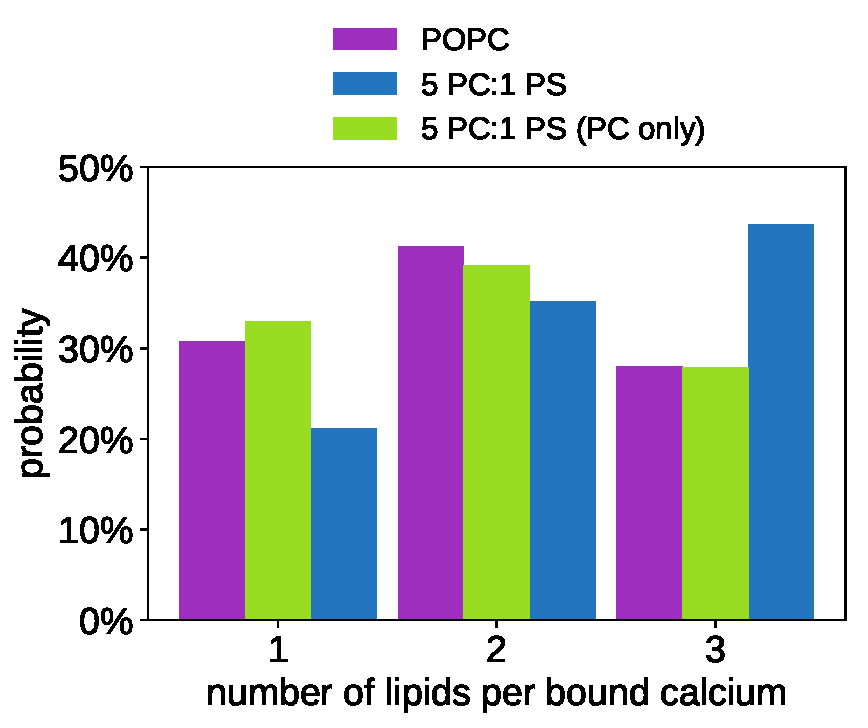
\includegraphics[width=\figwidth]{../img/stoichiometry_CaCl2_comparison_Ecc-lipids_PC-vs-PCPS.pdf} \\ 
  \caption{\label{fig:cacl_complexes} 
      Relative probabilities of existence of \ce{Ca^{2+}} complexes 
      with a certain number of lipids.  
      All lipids were taken into account with the exception of the complexes in light green, 
      for which we counted only contacts with POPC from the mixed 5\,PC:1\,PS negatively charged bilayer 
      and calculated the probabilities of the calcium-lipid complexes also only per POPC. 
      Probabilities were taken from simulations with comparable bulk concentrations of calcium around 250~mM. 
  } 
\end{figure} 
 



\subsection{Molecular interaction and binding affinities of Ca$^{2+}$  cations to the mixed POPC:POPS (5:1) membrane} 


%\todo{Stationary distribution: Make a figure documenting the populations of bound \ce{Ca^{2+}} cations (like I have in the presentation) that would accompany Table \ref{tab:Ca_binding_PCPS}. 
%This will roughly correspond to the PC stoichiometry plot \ref{fig:cacl_complexes}. }

The affinity towards PC and PS lipids and some of their groups was evaluated 
by counting contacts between the cation and the oxygen atoms of the lipids
similarly as was done in \cite{melcr18}. 
The threshold for counting a contact was set to be $0.3 \mathrm{nm}$, 
which encompasses the first peak of radial distribution function between the cations and the oxygen atoms of the lipids. 
%\todo{Show a figure of RDF documenting this?}

The percentages of the populations of membrane-bound calcium cations for various membrane moieties 
are summarized in Table~\ref{tab:Ca_binding_PCPS}.
Although the lipid ratio in the membrane is 5~PC:1~PS,
approximately half of the total population of bound calcium cations is in contact with PS lipids
with 7\% bound only to them. 
This corroborates the intrinsincally higher affinity of PS lipids to calcium cations compared to PC lipids. 

Cations that are bound only to PC in the mixed bilayer with PS 
behave similarly as in the pure PC bilayer
maintaining similar probabilities for clustering one, two or even three PC lipids together. 

The population analysis also suggests 
that the calcium cations prefer to reside in the phosphate region of the membrane. 
%Such a finding is further validated with a more detailed analysis using Markov state modeling (MSM) \citep{Pande_MSM_paper} \todoi{Add papers reviewing MSM, e.g. recent Pande's paper.}. 
%The set of states of a calcium cation 
%encompassed all possible combinations of up to three surrounding lipids. 
%In the case of PC, we used only the phosphate moitety, which forms the dominant contribution for calcium binding.
%For PS we also distinguished configurations in which calcium interacts with the carboxylate moiety. 
%All possible combinations of such states were used to build a Markov model at a lag time $25\,\mathrm{ns}$ using pyEMMA code by \citet{pyemma} \todoi{add citation for pyemma}. 
%The resulting MSM was validated using Chapman-Kolmogorov test \citep{FrankNoe_papers_MSM} \todoi{Add citation for Noe's papers on MSM, especially Chapman Kolmogorov test.}. 
%The stationary distribution of the states reveals a strong preference of the calcium cations to reside in the phosphate region of the mixed PC-PS membrane. 
%When interacting with PS, configurations with the phosphate moiety from either PC or PS dominate the population.
%Moreover, states containing interactions with the carboxylate group in PS 
%bear higher probability when interacting also with the phosphate group of the same lipid or other lipids. 
This is also reflected as a shift of the mean orientation of the \ce{COO^-} group from $62^\circ$ to $73^\circ$ (420~mM \ce{CaCl2})
measured as the connector of the carbon atoms, which form the bond between the group and the $\beta$-carbon of the phospholipid. 
The interactions of the carboxylate group in PS with calcium and other phosphate groups
sheds light into the qualitatively different response of the head group order parameters $\alpha$ and $\beta$ in PS compared to PC 
(see Figs.~\ref{fig:delta_ordPar_CaCl} and~\ref{fig:delta_ordPar_CaCl_PCPS}). 



The increased response of head group order parameters $\alpha$ and $\beta$ of PC, which form the lipid electrometer concept,
in mixed 5~PC:1~PS bilayer compared to pure PC
is due to higer affinity of the membrane mediated by even a relatively small fraction (1/6) of PS lipids. 
This is in line with the steep onset of the response of the PS head group order parameters at lower concentrations.
The complex response of the head group order parameters of PS lipids 
is due to the confomational change of the carboxylate group that is attracted more towards the phosphate region. 



\begin{figure}[tb!]
  \centering
  \hfill
\subfloat[neutral PC bilayer]{
  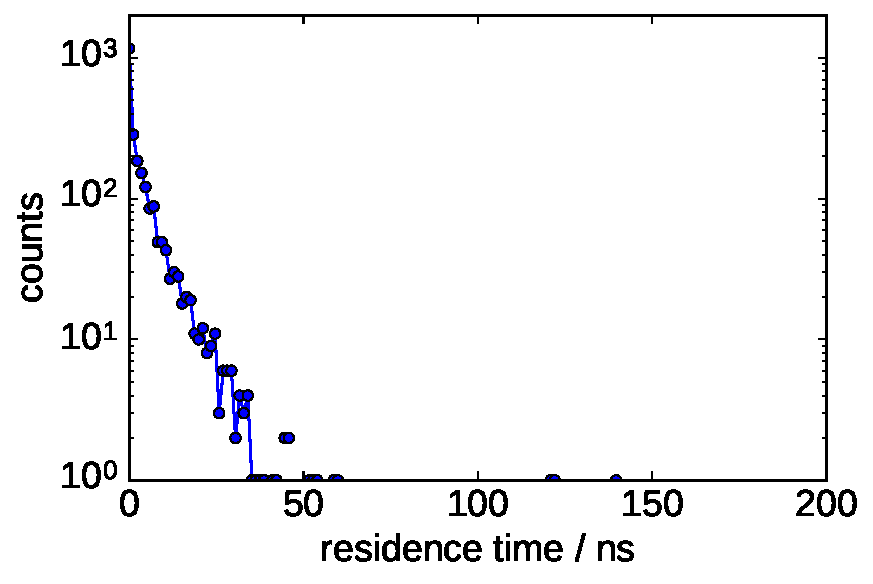
\includegraphics[width=\figwidthsmall]{../img/ecc_popc/histogram_bound_times_ECC-lipids_346mM_CaCl.pdf} 
}\hfill
\subfloat[negatively charged 5\,PC:1\,PS bilayer]{
  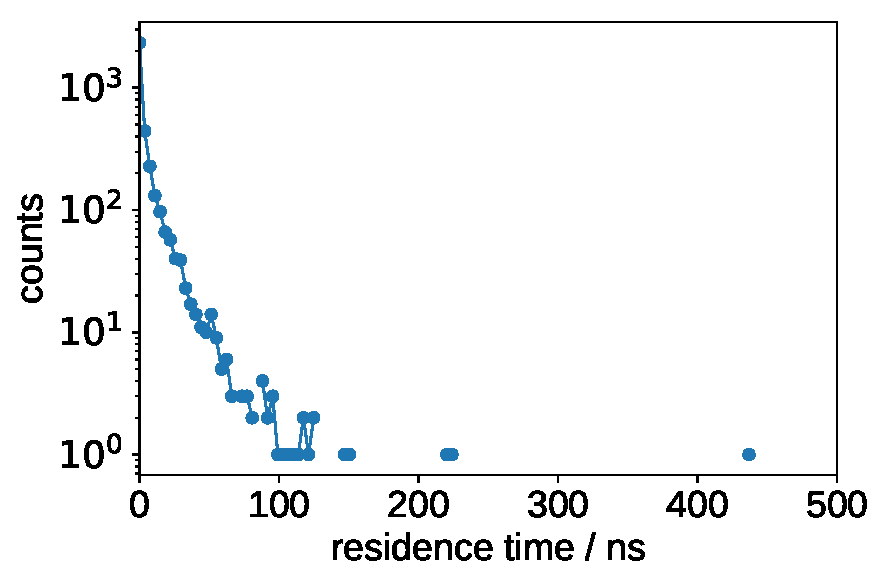
\includegraphics[width=\figwidthsmall]{../img/ecc_pops/histogram_bound_times_26CaCl2.pdf}
}\hfill
  \hfill
\todo{Put the scale of the x-axis the same -- or even better -- combine the plots into one!}
  \caption{\label{fig:hist_residence_times}
   Histograms of residence times of \ce{Ca^{2+}} 
   in a neutral membrane composed of POPC (left)
   and in a negatively charged membrane with a compostion 5\,PC:1\,PS (right)
   from simulations with ECC-lipids and ECC-ions.
   The simulation with the neutral membrane has a bulk concentration of calcium $C_{ion} = 280\mathrm{mM}$, 
   the simulation with the negatively charged membrane has a bulk concentration of calcium $C_{ion} = 240\mathrm{mM}$. 
   In the simulation with the neutral membrane, 
   90\% of the residence times of calcium cations are
   shorter than $60\,\mathrm{ns}$, % exactly $53\,\mathrm{ns}$                                                                          
   with the longest observed residence time being $141\,\mathrm{ns}$. 
   In the simulation with the negatively charged membrane, 
   90\% of the residence times of calcium cations are
   shorter than $180\,\mathrm{ns}$, % exactly $53\,\mathrm{ns}$                                                                          
   with the longest observed residence time being $440\,\mathrm{ns}$. 
   }
\end{figure}


Timescales associated with the binding of calcium cation from solution to the membrane
are plotted for each binding event as a histogram in Fig.~\ref{fig:hist_residence_times}. 
Using these plots, we can estimate the upper bound for the residence time of a calcium cation 
to be lower than $60\,\mathrm{ns}$ for pure POPC neutral bilayer 
and shorter than $180\,\mathrm{ns}$ for the mixed 5\,PC:1\,PS negatively charged bilayer. 
The longest observed residence times in the simulations were $141\,\mathrm{ns}$ for the neutral membrane 
and $440\,\mathrm{ns}$ for the negatively charged membrane. 
Both estimates of the residence times come from simulations with comparable concentrations around $250\mathrm{mM}$;
the simulation with the neutral membrane has a bulk concentration of calcium $C_{ion} = 280\mathrm{mM}$, 
whereas the simulation with the negatively charged membrane has a bulk concentration of calcium $C_{ion} = 240\mathrm{mM}$. 

%In addition to such estimates of the time scales, we used the Markov model on top of the simulation with the negatviely charged mixed bilayer
%to calculate the time of the mean first passage of calcium from solution to the membrane (and in reverse) resulting in $55\,\mathrm{ns}$  ($165\,\mathrm{ns}$). 

%\todo{Fluxes: committor analysis, dominant fluxes (table and figure)}
%From the spectrum of the transition matrix, we also observe that 
%the slowest transitions are associated with the binding to two or three phosphate moieties from either PC or PS,
%which are also among the states with the highest probabilities.
%The net fluxes of calcium cations from solution to such states also form a large contribution to the total flux ($\approx 45\%$). 
%\todo{Make a table and a figure of the state probabilities and fluxes to support this statement.}. 
%Analysis of the possible binding pathways of calcium cations to the negatively charged mixed bilayer 
%reveal that the cations mostly enter the membrane bound states directly from solution 
%without complicated transitions at the time scales of the order of the lag time of the Markov state model, $25\,\mathrm{ns}$. 










 


 
\subsection{Molecular interactions between Ca$^{2+}$ cations and POPC oxygens} 
We analyzed the ratio of the number of calcium cations bound to either phosphate or carbonyl moieties and the total number of bound cations in our POPC bilayers as done previously in Ref.~\citep{javanainen17}. A maximum distance of 0.3~nm from any lipid oxygen is used to define a bound calcium. The results from ECC-POPC simulation in Table~\ref{tab:binding} show that almost all (99\%) of the bound Ca$^{2+}$ ions are in direct contact with phosphate oxygens. From these ions, only one third (32\%) also interacts with the carbonyl oxygens, while the interaction of calcium ions with carbonyl oxygens only is rare (1\%). The most abundand interaction scenarios between Ca$^{2+}$ ions and phosphate oxygens are visualized using the probability density isocontours in Fig.~\ref{fig:volmaps}. While higher concentrations of \ce{CaCl2} increase the number of contacts per lipid, the distribution of contacts between phosphate and carbonyl oxygens is not affected. 
 
\todo{Analyze the orientation of the carbonyls and plot it as a violin plot/probability density. Change the following discussion afterwards.}
In the case of POPC, the $C_2$ segment in {\it sn}-2 chain shows a low order parameter with a small forking as measured in experiments by \citet{seelig75,schindler75,gawrisch92}. 
This feature has been suggested to indicate that the carbonyl
of {\it sn}-2 chain is directed towards the water phase, in contrast to the
carbonyl in {\it sn}-1 chain, which would orient more along the bilayer
plane~\cite{seelig75,schindler75,gawrisch92}. This may be an important
feature for the ion binding details, which it is not fully reproduced by other
available lipid models~\cite{ollila16}.

 
In conclusion, the results suggest that calcium ions bind specifically to the phosphate oxygens, occasionally interacting also with the carbonyls of the PC lipids. This is in a qualitative agreement with previous conclusions from several experimental studies~\citep{hauser76, hauser78, herbette84, cevc90, binder02}. However, the present results suggest, in 
agreement with experiments, an overally weaker binding to the bilayer, in particular with a lower relative binding affinity to the carbonyls than inferred from previous MD simulation studies~\citep{bockmann03, bockmann04, melcrova16, javanainen17}. 

 
\subsection{Binding stoichiometry of \ce{Ca^{2+}} cations to POPC membrane} 
Simple binding models have been used previously to interpret the same experimental data \citep{altenbach84,macdonald87} as employed in this work to validate the simulation models (Fig.~\ref{fig:delta_ordPar_CaCl}). In particular, NMR data concerning the PC headgroup order parameters response and atomic absorption spectra were explained best using a ternary complex binding model with a binding stoichiometry of one \ce{Ca^{2+}} per two POPC lipids~\citep{altenbach84}. Nevertheless, a Langmuir adsorption model assuming a \ce{Ca^{2+}}:POPC stoichiometry of 1:1 also provided a good fit to the experimental data when considering \ce{CaCl2} at low concentrations only~\citep{macdonald87}. 
 
 
In this work, we reproduce the same experimental data used to infer binding stoichiometries employing our ECC-POPC model. Thanks to our simulations, we have a direct access to atomistic details of the binding stoichiometry without a need for any binding model as employed for interpreting in experiments~\citep{altenbach84, macdonald87}.
To evaluate the relative propensities for each of the stoichiometric complexes (i.e.,~1~Ca$^{2+}$:~n~POPC),
we calculated for each bound Ca$^{2+}$ the number of POPC molecules having oxygen atoms within a distance of 0.3~nm.
Results from the POPC bilayer simulation with a 285~mM bulk concentration of CaCl$_2$ are shown in Fig.~\ref{fig:cacl_complexes}. 
We found the largest propensity for the 1:2 complex (41\%), with probabilities of complexes with the stoichiometries of 1:1~(25\%)~and 1:3~(34\%)~being only slightly lower. This suggests a more complex binding model than considered in a simple 1:2 ternary complex model previously. Nevertheless, with a broad brushstroke, the simulation data can be viewed such that one calcium binds to two lipids on average, because the probabilities of the complexes with 1 or 3 lipids are almost equal to each other  (and complexes with more than three lipids per one calcium ion were not observed). This probably explains why the simple the ternary complex model fits adequately the experimental data, as well as the ECC-POPC simulation results (see Fig.~S3 in SI). 
 
 
 
\subsection{Residence times of \ce{Ca^{2+}} cations in the POPC membrane} 
 
Equilibration of \ce{Ca^{2+}} ions at a POPC bilayer in MD simulations is a microsecond time scale process with current force fields, such  as CHARMM36 and Slipids force fields~\citep{javanainen17}. This suggests that at least several microseconds are required to reach the ion binding/unbinding equilibrium. 
To quantify the exchange of ions between the membrane and aqueous solution in simulations, we evaluated residence times of ions bound to the membrane. Within our analysis, an ion is considered to be bound when it is within 0.3~nm from any oxygen atom belonging to a POPC molecule. 
 
The histograms of residence times of \ce{Ca^{2+}} in a POPC bilayer ($C_{ion}'$ = 450~mM) from simulations with  
ECC-POPC and CHARMM36 (simulation from Refs.~\citep{javanainen17,zenodo.259376}) are shown in Fig.~S4 in SI. 
In the CHARMM36 simulation, a significant number of the calcium ions is bound to the membrane for the whole length of the trajectory (800~ns). 
In contrast, at least an order of magnitude faster bound/unbound calcium exchange is observed within the ECC-POPC model, 
where 90\% of the \ce{Ca^{2+}} residence times to a POPC membrane are shorter than $60\,\mathrm{ns}$. The longest observed 
residence time is around 150~ns, which is below the total length of the simulation used for analysis, i.e., 200~ns. 
Note that these results are in line with the experimental estimate that the residence time of \ce{Ca^{2+}} at each PC 
headgroup is of the order of $10\,\mu\mathrm{s}$~\citep{altenbach84}. 
 
In summary, the results from the ECC-POPC model suggest that the exchange of calcium between the POPC bilayer and the solvent occurs within the $\sim$100~ns timeframe, which is significantly faster than observed in simulations emloying most of the presently available lipid models~\citep{javanainen17}. Sodium cations exhibit an even more rapid exchange between the membrane and the aqueous solution. Our results suggest that simulations with a length of several hundreds of nanoseconds are sufficient to simulate alkali and alkali earth ion binding to phospholipid bilayers in equilibrium when realistic force fields are used. This has not been the case with previous lipid force fields, which overestimate the binding strength of the sodium and, in particular,  calcium cations \citep{javanainen17, catte16}. 
 
 











\chapter*{Conclusion}
\addcontentsline{toc}{chapter}{Conclusion}

Motivated by cellular processes, 
which involve ions and cell membranes as major actors, 
we have investigated model phospholipid membranes and their interactions 
with biologically relevant ions. 
The controlled concentrations of \ce{Na^+} and \ce{K^+} cations 
on either side of the membrane of neurons
forms the transmembrane potential. 
Neurons vary the concentrations of theses cations
to modulate the transmembrane potential 
and to conduct electrical signals along the axons. \citep{Knudsen_book2002, Storace2015, Sung2015}
In our work \citep{melcr16},
we compared two methods for modeling of the transmembrane potential in molecular simulations, 
i.e., 
the constant electric field method \cite{Roux1997,Roux2008, gumbart_constant_2012}, 
and the ion imbalance method \cite{sachs04_potential, kutzner_computational_2011}. 
We have proven the two methodologies to be equivalent, 
at least for electrolytes formed by the same monovalent ions on both sides of the membrane. 
%This was demonstrated by simulations, 
%in which we simultaneously applied both methods
%with an opposite polarity. 
%The results from such a setup were indistinguishable 
%from simulations without voltage within the achievable accuracy. 
While
the structure of the bilayer remains almost unchanged by the transmembrane potential, 
the induced electric field in the hydrophobic core of the bilayer
affects the orientation of water molecules at its interface 
highlighting its importance in electroporation. \citep{bu2017mechanics}


Next,
we performed extensive sets of simulations of phospholipid bilayers
with different salts at varying concentrations
to study the binding of cations to model membranes. 
We used the most abundant representants of phospholipids
to form neutral (POPC) or negatively charged (5\,POPC:1\,POPS) bilayers, 
for which we have provided a detailed insight 
into the interactions with 
\ce{Na^+}, \ce{K^+}, and \ce{Ca^{2+}} cations. 
The affinity of the cations 
was measured using the concept of a lipid electrometer 
introduced by \citet{seelig87} 
and described in section~\ref{section:electrometer}.
The head group order parameters $\alpha$ and $\beta$ in POPC
%(see Fig.~\ref{fig:simVSexpNOions} for the definition of the order parameters)
are experimentally observed to change
proportionally to the bound charge per lipid. 
Such changes can then be related to the amount of bound ions.

In our publications \citep{catte16, nmrlipids_proj4},
we have shown that such order parameters can be accurately determined also from MD simulations
and their changes correlate with the amount of bound charge in phospholipid bilayers, 
despite the inaccuracies in their actual structures without salts \citep{botan15}. 
It was found, however, that
none of the force fields examined in those works 
provided a sufficient accuracy for interpreting 
the experimentally measured structural changes induced by salt concentrations
and cation-lipid stoichiometries. 
While there were several models
that predicted realistic binding affinities of \ce{Na^+} to PC bilayers,
all existing models overestimated the binding affinity of \ce{Ca^{2+}}
unless ad hoc specific repulsive potentials between the cations and the bilayer were applied. \citep{catte16, nmrlipids_proj4}
Thus,
we identified the strong binding of \ce{Na^+} and \ce{Ca^{2+}} cations
in existing simulation models as a computational artifact.  
Such excessive amounts of cations 
would form effectively positively charged membranes
even at physiological concentrations
affecting interactions with any charged molecules. 
For instance,
the total charge of proteins
in prokaryotes and also eukaryotes 
is mostly negative,
\citep{link1997identifying, link1997comparing, urquhart1998comparison, schwartz2001whole, knight2004global}
Thus,
positively charged membranes would promote non-specific adsorption of proteins on their surface 
contrary to experiment.  
\citep{junkova2016, lingwood2010lipid, sekerevs2015song} 


A major improvement over currently available non-polarizable force fields
was achieved by developing new models of phospholipids, 
the so called ECC-lipids,
which are described in section~\ref{section:ecc-lipids}
and in the publication \citep{melcr18}. 
In contrast to the models studied in the works \citep{catte16, nmrlipids_proj4},
ECC-lipids account for electronic polarization
via the electronic continuum correction,  
which was introduced in section~\ref{section:ecc}. 
In short, 
ECC is an implicit model of electronic polarizability,
which can be straightforwardly implemented into current force fields 
by scaling charges.  
In section~\ref{section:ecc-lipids},
we demonstrated on the cases of PC, PS, and PE phospholipids
that it is sufficient to also scale the Lennard-Jones parameters $\sigma$ of the affected atoms
to reach a structural agreement with x-ray scattering experiments. 
Our new model, ECC-lipids,
provides a proof of concept of the applicability of ECC
to charged as well as neutral molecules. 



Our simulations with ECC-lipids suggest that
\ce{Na^+} and \ce{Ca^{2+}} cations
interact specifically with the phosphate and carboxylate groups of PC and PS 
and occasionally also with the carbonyl groups. 
\ce{K^+} interacts only very weakly with the bilayers
affecting slightly only carboxylate groups in POPS,
which are more exposed to the solvent compared to phosphate groups. 
In overall, weaker binding of cations to phospholipid bilayers is observed 
compared to previous MD simulation studies~\citep{nmrlipids_proj4, catte16, bockmann03, bockmann04, melcrova16, javanainen17}. 
Importantly,
our simulations show for the first time a \emph{quantitative} agreement with the experimental lipid electrometer concept
for POPC and also for POPS with all the studied cations. 
For instance, the small differences 
in the responses of the order parameter $\beta$ in POPS
between the 
\ce{Na^+}, \ce{K^+}, and \ce{Ca^{2+}} cations
are captured well by our model. 
Also, the exchange of calcium between a phospholipid bilayer and solvent 
occurs at the order of 10--100~ns, 
which is in accord with experiments and also 
significantly faster than the time scales from simulations 
with other presently available non-polarizable models of lipids~\citep{melcrova16, javanainen17, catte16}. 
Nevertheless, even with ECC-lipids,
the reversible process of calcium binding to phospholipid bilayers in equilibrium
requires simulations of a characteristic length of several hundreds of nanoseconds 
for the neutral bilayers,
while almost an order of magnitude longer lengths 
are required for the negatively charged bilayers. 
In summary,
our results are in accordance with the works,
which suggest that monovalent cations (with the exception of \ce{Li^+}) 
exhibit negligible binding to phospholipid bilayers, 
while multivalent cations interact significantly 
\citep{cevc90,tocanne90, hauser76,hauser78,herbette84,altenbach84,clarke99,binder02,pabst07,uhrikova08,filippov09}.


Treatment  of the electronic polarization 
was shown to have a dramatically positive impact on the accuracy of the description of interactions
between phospholipids and cations. 
The presented application of ECC to lipids
constitutes a pivotal work for its future adaptations 
to also other compounds, especially charged and zwitterionic, 
e.g., proteins or nucleic acids,
for which we expect improvements in computational description in a similar range. 



%%% Bibliography
%%% Bibliography (literature used as a source)
%%%
%%% We employ bibTeX to construct the bibliography. It processes
%%% citations in the text (e.g., the \cite{...} macro) and looks up
%%% relevant entries in the bibliography.bib file.
%%%
%%% The \bibliographystyle command selects, which style will be used
%%% for references from the text. The argument in curly brackets is
%%% the name of the corresponding style file (*.bst). Both styles
%%% mentioned in this template are included in LaTeX distributions.

\bibliographystyle{plainnat}    %% Author (year)
% \bibliographystyle{unsrt}     %% [number]

\renewcommand{\bibname}{Bibliography}

%%% Generate the bibliography. Beware that if you cited no works,
%%% the empty list will be omitted completely.

\bibliography{bibliography}

%%% If case you prefer to write the bibliography manually (without bibTeX),
%%% you can use the following. Please follow the ISO 690 standard and
%%% citation conventions of your field of research.

% \begin{thebibliography}{99}
%
% \bibitem{lamport94}
%   {\sc Lamport,} Leslie.
%   \emph{\LaTeX: A Document Preparation System}.
%   2nd edition.
%   Massachusetts: Addison Wesley, 1994.
%   ISBN 0-201-52983-1.
%
% \end{thebibliography}


%%% Figures used in the thesis (consider if this is needed)
\listoffigures

%%% Tables used in the thesis (consider if this is needed)
%%% In mathematical theses, it could be better to move the list of tables to the beginning of the thesis.
\listoftables

%%% Abbreviations used in the thesis, if any, including their explanation
%%% In mathematical theses, it could be better to move the list of abbreviations to the beginning of the thesis.
\chapwithtoc{List of Abbreviations}

\begin{description}   %[align=right]  ,labelwidth=3cm]
\item [MD]   Molecular dynamics
\item [ECC]  Electronic continuum correction
\item [POPC] Palmitoyloleoylphosphatidylcholine
\item [DPPC] Dipalmitoylphosphatidylcholine
\item [POPS] Palmitoyloleoylphosphatidylserine
\item [POPE] Palmitoyloleoylphosphatidylethanolamine
\item [PC]   Phosphatidylcholine
\item [PS]   Phosphatidylserine
\item [PE]   Phosphatidylethanolamine
%\item [MSM]  Markov state modeling
\item [NMR]  Nuclear Magnetic Resonance
\end{description}

%%% Doctoral theses must contain a list of author's publications
\chapwithtoc{List of publications and attachments}

%%% Attachments to the doctoral thesis, if any. Each attachment must be
%%% referred to at least once from the text of the thesis. Attachments
%%% are numbered.
%%%
%%% The printed version should preferably contain attachments, which can be
%%% read (additional tables and charts, supplementary text, examples of
%%% program output, etc.). The electronic version is more suited for attachments
%%% which will likely be used in an electronic form rather than read (program
%%% source code, data files, interactive charts, etc.). Electronic attachments
%%% should be uploaded to SIS and optionally also included in the thesis on a~CD/DVD.
%%% Allowed file formats are specified in provision of the rector no. 72/2017.
%\chapter{Attachments}

\begin{itemize}
% paper Transmembrane potential modeling, JCTC 2016
\item[I] 
Transmembrane Potential Modeling: Comparison between Methods of Constant Electric
Field and Ion Imbalance. 
Journal of Chemical Theory and Computation, 12(5), (2016). 
Josef Melcr, Daniel Bonhenry, Štěpán Timr, and Pavel Jungwirth. 

% paper NMRLipids II project -- lipid-ion interaction PCCP 2016
\item[II] 
Molecular electrometer and binding of cations to phospholipid bilayers. 
Phys. Chem. Chem. Phys., (2016).
Andrea Catte, Mykhailo Girych, Matti Javanainen, Claire Loison, Josef Melcr,
Markus S. Miettinen, Luca Monticelli, Jukka Maatta, Vasily S. Oganesyan,
O. H. Samuli Ollila, Joona Tynkkynen, and Sergey Vilov. 

\item[III]
Accurate Binding of Sodium and Calcium to a POPC Bilayer by Effective Inclusion of Electronic Polarization. (2018)
The Journal of Physical Chemistry B, 122(16), (2018).
Josef Melcr, Hector Martinez-Seara, Ricky Nencini, Jiří Kolafa, Pavel Jungwirth,
and O. H. Samuli Ollila. 

\item[IV]
Head group and glycerol backbone structures,
and cation binding in bilayers with PS lipids. (2018)
Amelie Bacle, Pavel Buslaev, Lukasz Cwiklik, Fernando Favela, Tiago Ferreira,
Patrick Fuchs, Ivan Gushchin, Matti Javanainen, Batuhan Kav, Jesper Madsen, 
Josef Melcr, Markus Miettinen, Ricky Nencini,  Chris Papadopoulos, Thomas Piggot 
and O. H. Samuli Ollila. 

\end{itemize}

\appendix

\openright
\end{document}
